\documentclass[11pt]{article}
\usepackage[letterpaper]{geometry}
\usepackage{amsthm,amsmath,amsfonts}

\usepackage{color,graphicx}
\usepackage{float}
\usepackage[colorlinks]{hyperref}
\newcommand{\red}[1]{\textcolor{red}{#1}}
\newcommand{\blue}[1]{\textcolor{blue}{#1}}
\usepackage{natbib}
\usepackage{centernot}
\usepackage{enumerate}
\newcommand{\R}{\mathbb{R}}
\newcommand{\D}{\mathbb{D}}
\newcommand{\C}{\mathbb{C}}
\newcommand{\Z}{\mathbb{Z}}
\newcommand{\I}{\mathbb{I}}
\newcommand{\E}{\mathbb{E}}
\newcommand{\N}{\mathbb{N}}
\newcommand{\Prob}{\mathbb{P}}
\usepackage{graphicx}
\graphicspath{ {images/} }
\providecommand{\abs}[1]{\lvert#1\rvert}
\providecommand{\argmin}{\text{argmin}}
\providecommand{\norm}[1]{\lVert#1\rVert}
\newtheorem{lemma}{Lemma}
\newtheorem{theorem}{Theorem}
\newtheorem{corollary}{Corollary}
\newtheorem{remark}{Remark}
\theoremstyle{definition}
\numberwithin{equation}{section}
\newtheorem{definition}{Definition}
\newtheorem{assumption}{Assumption}
\newtheorem{example}{Example}
\usepackage{tikz}
 \usepackage{tkz-graph}
 \usetikzlibrary{arrows}
\usetikzlibrary{positioning}
\usetikzlibrary{calc,fit}
\usepackage[font=small, labelfont=bf]{caption}
\usepackage{subfig}
\usepackage{float}
\usepackage[ruled,vlined,linesnumbered]{algorithm2e}
\begin{document}
\begin{center}
  \large \bf
Multiclass Queueing Networks Scheduling Optimization Using Deep Reinforcement Learning
\end{center}
\begin{center}
  Mark Gluzman \\
  7/11/2019
\end{center}






\section{Introduction}



In recent years deep reinforcement learning (RL) has become extremely popular research area in AI community with real-world impact. Decision strategies obtained from RL algorithms outperform human in one-player games \cite{Bellemare2013, Mnih2015}, two-players games \cite{Silver2017},  team games \cite{OpenAI2019}; are successful in wide range applications from medicine \cite{Komorowski2018} to  cooling datacenters \cite{DeepMind2016a}. Following the trend many dynamic resource allocation and sequential decision making problems in communications and networking are solved applying deep RL, see the review \cite{CongLuong}.



 One of the hard problems in stochastic processing networks domain is the optimization scheduling policies for multiclass queueing networks (MQNs). % MQNs arise in service, communication, and manufacturing systems
 In the scheduling optimization problem the decision maker determines which job class should be precessed first in each node (server) of the system.

One approach to optimize scheduling policies is to assume that the multiclass queueing networks is heavily
loaded. Then the original scheduling problem can be approximated by a reflected Brownian motion (RBM) \cite{Harrison1988, Harrison1989, Wein1990}.  However, determining the stationary distribution of the reflected Brownian motion in higher than two dimensions is hard and, except the cases with state-space collapse \cite{Williams1998, Laws1990}, this approach is untractable for higher dimensions.

Another approach is to consider fluid model approximations. The strong connection between stability of multiclass queuing network and the associated fluid model has been shown in \cite{Dai1995}. There are several papers where authors develop methods to
translate a policy derived from fluid optimal control problem into a policy for the original stochastic processing network, for example affine shift policies \cite{Meyn1997}, discrete-review policies \cite{Maglaras2000}, and tracking policies \cite{Bauerle2001a}.

 While fluid models are more tractable than RBM, they ignore the ``variance'' of the associated original stochastic processing network.   In \cite{Bertsimas2015} the authors propose to assume that realization
of the arrival rates and service times can deviate from their mean values in some pre-set interval. The method allows to inject uncertainty in the fluid model. The optimization problem  based on a new robust fluid model remains trackable for large multiclass networks. Each decision epoch the decision maker formulates and solves a robust fluid optimization problem for a current system state. It requires knowledge of nominal mean arrival rates and service times, as well as routing probabilities.


 For the queuing networks with Poisson arrival and exponential service time assumptions the control problem can be modeled within the framework of Markov decision processes (MDPs) via uniformization.   Based on information that is available for the system manager we distinguish two approaches of solving MDPs: approximate dynamic programming and reinforcement learning.


 In dynamic programming paradigm the decision maker has full knowledge about the MDP problem (transition probabilities, cost-to-go function, etc.).
 A fundamental difficulty in solving the MDP problem directly  is the curse of dimensionality: the buffers capacity is unlimited and the corresponding optimization
problem has infinite number of constrains and unknowns. Even if the number of waiting jobs in each buffer is limited, the
complexity of the problem grows exponentially with the number of job classes. Approximate dynamic programming (ADP)  aims to approximate the original MDP to make the problem computationally trackable and yet obtain near optimal control policies. Usually additional assumptions on the value function structure are imposed, see \cite{DeFarias2003a, Abbasi_Yadkori2014a, Veatch2015}.

In practice the system manager may not have full information about arrival, service processing rates and routing path of each job class. The goal of  reinforcement learning algorithm is to find near-optimal  policies when a probabilistic model of the system is not provided, and only the current state of the queuing network is known. %The performance in such problems is evaluated and optimized  through stochastic simulations.


The following RL methods have been applied for queuing scheduling control problem: look-up table Q-learning \cite{Ramirez-Hernandez}, SARSA($\lambda$) with linear Q-functions representation \cite{Ramirez-Hernandez2007a},  actor-critic method \cite{Ramirez-Hernandez2007c}, policy gradient \cite{Paschalidis2004}, MCTS \cite{Bertsimas2017}. Except the last paper, only small networks with no more than six job classes have been considered. In \cite{Bertsimas2017} the MCTS method has been compared with fluid network approach \cite{Bertsimas2015} and shown similar or worse results.

In this paper we describe an iterative deep RL algorithm that can be classified as a  conservative policy iteration algorithm \cite{Kakade2002}. Conservative policy iteration algorithms find a gradient direction that  guarantees monotonic improvement of a current policy, but constrain the magnitude of policy update to omit performance collapse caused by large changes in the policy.
In  \cite{Schulman2015} the authors prove that minimizing a certain surrogate objective function guarantees decreasing of expected discounted cost. Unfortunately, the theoretically-justified step-sizes of policy updates cannot be computed from available information for the RL algorithm.  Trust Region Policy Optimization (TRPO) \cite{Schulman2015} has been proposed as a practical method to restrict policy updates. Proximal policy optimization (PPO) is an alternative way of adjusting step-sizes based on clipped surrogate objective \cite{Schulman2017}. %It is simpler to implement, claimed to have better sample complexity and outperform TRPO on the popular benchmarks.

 In Section \ref{sec:TRPOforAC} we provide theoretical justification that minimizing  surrogate objective function with cost discounting can guarantee monotonic decrease of the long-run average cost. In Section \ref{sec:Algorithm} we describe in details practical modifications to the algorithm, including PPO step-size control.


We mostly compare performance of our RL policies with the performance of robust fluid policies reported in \cite{Bertsimas2015}.  Robust fluid policies yield performance that is near-optimal for small-size networks, and have better performance for moderate and large-size networks in comparison with  the best other heuristic policies. We want to note several differences in the problem formulation for a RL algorithm and robust fluid optimization problem:
\begin{itemize}
\item robust fluid problem requires knowledge of all parameters of the system including mean arrival rates,  mean service times, routing probabilities and cost of each transition. In the RL framework no information about transition probabilities and cost-to-go function  is assumed to be available.
\item RL algorithms rely on simulations of multiple policies. We assume that a simulation environment is available for the decision maker. Such simulation environment can be a real system or a virtual/generative model.
\end{itemize}





We summarize the major conclusions from our study:
\begin{enumerate}
  \item We propose a reinforcement learning method based on  PPO \cite{Schulman2017} algorithm for the multiclass processing network control problem. To the best of our knowledge, this is the first paper which proposes an algorithm for average number of jobs minimization that is trackable and does not require first-order system data (arrival rates, mean processing
times, and routing probabilities).

\item We provide an iterative procedure for minimizing long-run average cost based on advantage function with discounted future costs, with guaranteed monotonic improvement. We  discuss several approximations to the
theoretically-justified procedure to get a practical algorithm.



  \item We provide extensive computational experiments and claim the following:
   \begin{enumerate}
     \item The performance of RL policies is comparable with model-based fluid network approach  \cite{Bertsimas2015}, \cite{Bertsimas2017} and better than baseline heuristics.
     \item The choice of hyperparametrs (such as number of episodes, their duration, discount factor, clipping parameter, etc.) can   affect convergence of the algorithm and performance of RL policies. We provide guidance how to choose  hyperparametres.
         \item We propose  a neural network architecture that effectively parameterizes scheduling policies.
   \end{enumerate}



  %\item In the average reward setting it is unclear where to initialize the episodes. We compare three techniques, that start every episode by resetting to: 1) a state from a demonstration (given trajectory) of a stable policy, 2)  fixed initial state, i.e. empty system, 3) a state visited during the latest episode simulations.
\end{enumerate}


\section{Control of multiclass queueing networks}\label{sec:MQN}

In this section we formulate the scheduling control problem for multiclass processing networks. We first give the optimal control problem formulation for the criss-cross network  and then describe the
formulation of the problem for a general multiclass queueing network.


\subsection{The criss-cross network}
The criss-cross network has been considered in \cite{Harrison1990} and depicted in Figure  \ref{fig:cc}. It consists of two stations that process three classes of jobs. Each job class  has its own affiliated buffer where jobs wait to be served.

\begin{figure}[h]
\centering%
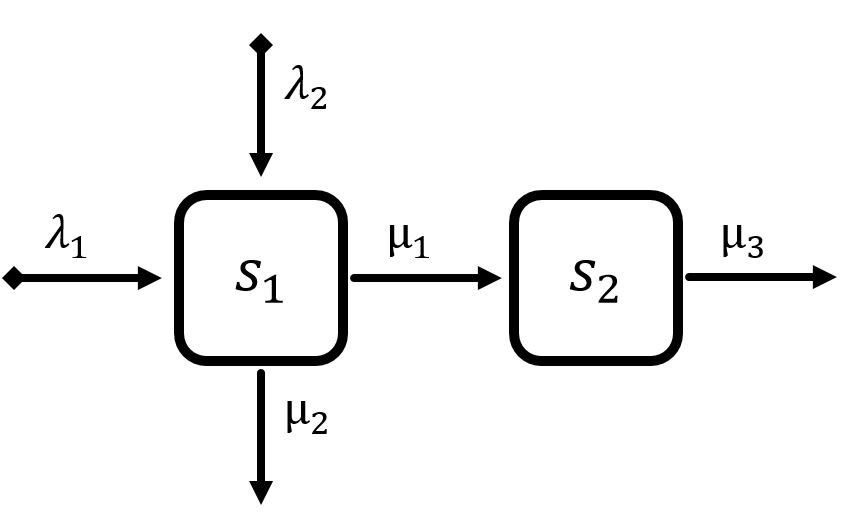
\includegraphics[width=.6\linewidth]{Paper_criss_cross.JPG}
\caption[]{The criss-cross network}
\label{fig:cc}%
\end{figure}

 We assume that the jobs of class 1 and class 2 arrive to the system following Poisson process with rate $\lambda_1$ and with rate $\lambda_2$ correspondingly. Both classes are served in the 1st server. After being served jobs of class 1 become jobs of class 3 and wait for 2nd server service. Jobs of the 2nd and 3rd classes leave the system after their service completion.
Service times are i.i.d. having exponential distribution with mean $m_j,~ j = 1, 2, 3$.



We assume that both servers employ an non-idling service policy, which means that each
server must be busy whenever there is a job available for processing. The only decision that the system manager has to make is to choose whether to process a job of class 1  or a job of class
3 if both buffers 1 and 3 are non-empty.

Let $x_j(t)$ be the number of class $i$ jobs (including possibly the one in service) in the system  at
time $t,~j = 1, 2, 3$.  We use $x(t) = \left[x_1(t), x_2(t), x_3(t)\right]$ to denote the system state at time $t$. We assume that the system manager executes a stationary Markovian policy $\pi$ i.e. the policy $\pi$ dictates a preemption-resume priority for jobs of either class 1 or class 3 solely based on the system state $x(t)$ at time $t$.


 The objective is to find a stationary policy that minimizes the long-run average number
of jobs in the network:

\begin{equation}\label{co}
\inf\limits_{\pi} \lim\limits_{T\rightarrow \infty} \frac{1}{T} \underset{\pi}{\E} \int\limits_0^T\Big[x_1(t)+x_2(t)+x_3(t)\Big]dt
\end{equation}

Under classical assumptions on arrival and service processes we can convert the original continuous-time problem to  an equivalent continuous-time Markov process where the average time between
transitions is constant. The problem becomes  probabilistically equivalent to   discrete-time control
problem \cite{Lippman1975}.


 We let $\nu = \lambda_1+\lambda_2 + \sum\limits_{i=1}^3 \mu_i$  denote uniform transition rate, where $\mu_i = \frac{1}{m_i}$, $i=1, 2, 3$. We can consider the equivalent discrete-time control
problem, where depending on control, $a = 1$ (class 1 has preemption-resume high priority) or $a = 2$, the transition probabilities are given by:



\begin{equation}\label{eq:pr}
        \begin{aligned}[b]
&P_{(x_1, x_2, x_3),(x_1-1, x_2, x_3) }(a=1) = \frac{\mu_1}{\nu}1_{x_1>0}\\
&P_{(x_1, x_2, x_3),(x_1, x_2-1, x_3) }(a=1) = \frac{\mu_2}{\nu}1_{x_2>0, x_1=0}\\
&P_{(x_1, x_2, x_3),(x_1-1, x_2, x_3) }(a=2) = \frac{\mu_1}{\nu}1_{x_1>0, x_2=0}\\
&P_{(x_1, x_2, x_3),(x_1, x_2-1, x_3) }(a=2) = \frac{\mu_2}{\nu}1_{x_2>0}\\
&P_{(x_1, x_2, x_3),(x_1+1, x_2, x_3) } = \frac{\lambda_1}{\nu}\\
&P_{(x_1, x_2, x_3),(x_1, x_2+1, x_3) } = \frac{\lambda_2}{\nu}\\
&P_{(x_1, x_2, x_3),(x_1, x_2, x_3-1) } = \frac{\mu_3}{\nu}
        \end{aligned}
\end{equation}

The probability of having a fictitious transition is
\begin{align*}
&P_{(x_1, x_2, x_3),(x_1, x_2, x_3) } = 1 - P_{(x_1, x_2, x_3),(x_1+1, x_2, x_3) } - \\
&\quad\quad\quad P_{(x_1, x_2, x_3),(x_1, x_2+1, x_3) } - P_{(x_1, x_2, x_3),(x_1-1, x_2, x_3) } - P_{(x_1, x_2, x_3),(x_1, x_2-1, x_3) }-P_{(x_1, x_2, x_3),(x_1, x_2, x_3-1) }
\end{align*}

The "fake" event  does not
represent any real jump in the original CTMC, but allows to unify average time between real
transitions.

We abuse the notation and denote a state  as $x(k) = [x_1(k), x_2(k), x_3(k)]$ after $k$ transitions of the DTMC.


The objective (\ref{co}) is equivalent to:
\begin{equation}\inf\limits_{\pi} \sum\limits_{N\rightarrow \infty}\frac{1}{N}\underset{\pi}{\E}\left[ \sum\limits_{k=0}^{N-1}(x_1(k)+x_2(k)+x_3(k))\right].\end{equation}





\subsection{General formulation}




Let $L$ be a total number of services and $I$ be the total number of buffers.  We let $x(t) = [x_1(t), x_2(t), ..., x_J(t)]$ denote the number of jobs of each class $i$ at time $t$ in the system, including a job that might be in service. We interpret $s(i)$ as the server associated with job class $i$. We define $B_l = \{j, j=1, .., J:~ s(j)  = l\}$ as a set of classes that are processed by server $l$. We assume that routing in the network can be probabilistic: after being served  job of class $j$ becomes job of  class $k$ with probability $u_{jk}$ and leave the network with probability $1 - \sum\limits_{k=1}^K u_{jk}.$ We let $J\times J$ matrix $U = (u_{mn})_{m,n=1,..., J}$ denote the routing probabilities. External arrival processes are Poisson with rate $\lambda_j$ for jobs of class $j$, $j=1, .., J$. If no  external arrivals enter $j$th buffer we take $\lambda_j=0$. Class $j$ service times are i.i.d. having exponential
distribution with mean $1/\mu_j$, $j=1, ..., J$.


For each class $j = 1, .., J$, let $\alpha_j$ be the total arrival rate
into buffer $j$, that besides external arrivals involves transitions of jobs into class $j$ from
other classes. The vector $\alpha = [\alpha_1, \alpha_2, ..., \alpha_J]$ satisfies the following system of linear
equations, usually called as traffic equations: \begin{equation}\alpha = \lambda +U^T\alpha.\end{equation} We define the utilization of server $l$ as \begin{equation}\rho_l = \sum\limits_{j\in B_l} \frac{\alpha_j}{\mu_j}.\end{equation}
We assume that $\rho_l<1$ for all  services $l = 1, ..., L$.

 The objective is to find a stationary Markovian policy  $\pi$ that   minimize the expected long-run average number of jobs in the system:

\begin{equation}
 \inf\limits_\pi \lim\limits_{T\rightarrow \infty} \frac{1}{T} \E_{\pi}\Big[\int\limits_{0}^{T-1}\sum\limits_{j=1}^J x_j(t)dt\Big]
\end{equation}


We use uniformization to formulate MDP problem with state space $X = \mathbb{Z}_+^J$.

%We let $\nu = \sum\limits_{i=1}^I \lambda_i + \sum\limits_{i=1}^I \mu_i$  denote uniform transition rate.
We let $a_j(k)$  denote a control at $k$th decision epoch that provides priority to $j$th class, i.e. $a_j(k)=1$ means that class $j$ has the priority over other associated to server $s(j)$ classes to be served right after $k$th decision epoch. We note that $\sum\limits_{j \in B_l} a_j(k)=1$ for each server $l=1, .., L$ at each time-step $k=0, 1, 2....$  We denote the action space of the MDP problem as $A$.


The objective of the MDP problem  is to find a stationary Markovian policy $\pi:X\rightarrow A$ that minimizes long-run average number of jobs in the system, namely:

\begin{equation}
 \inf\limits_\pi \lim\limits_{N\rightarrow \infty} \frac{1}{N} \E_{\pi}\Big[\sum\limits_{k=0}^{N-1}\sum\limits_{j=1}^J x_j(k)\Big]
\end{equation}





\section{Reinforcement learning approach for queuing network control}

The undeniable success of RL has been reached for games \cite{Mnih2015}, \cite{Bellemare2013}, and physics engines \cite{Duan2016},  \cite{Todorov2012}. These problems are episodic in nature and have long but finite horizon. In the game domain each new episode (game) may require a different amount of time for the player to finish. To compare the effect of different actions  the objective is
normalized by discounting future costs.
  Many algorithms, including TRPO and PPO, have been designed to optimize the infinite horizon discounted total cost.

In some domains, for example stochastic processing networks, it is more appropriate to optimize the long-run average cost.
As has been noted in \cite{Thomas} many actor-critic algorithms, that claim to solve discounted cost minimization problem,  can be more  appropriate to solve average cost problems. Once initial states for the episodes are sampled from a stationary distribution of a current policy, the discounted total cost is proportional to the average performance of the the policy, see Theorem \ref{Vnu} in Section \ref{sec:proofs}.






In this section we  argue that our version of Proximal Policy Optimization algorithm is appropriate to optimize  the long-run average performance, even with discounting  future costs.

\subsection{Monotonic improvement guarantee for average cost objective}\label{sec:TRPOforAC}




%We first consider the average cost problem for finite state space and then discuss possible generalization for countable state space.


Consider a MDP problem with finite state space $X$, action state $A$, one-step cost function $g(x,a)$ and transition kernel $P(\cdot|x, a)$.


\begin{definition}

We denote the long-run average cost  of policy $\pi$ as
\begin{equation}
\eta_\pi = \underset{\substack{x\sim \mu_\pi\\ a\sim \pi(\cdot|x)}}{\E} g(x,a),
\end{equation}
where  $g(x,a)$ is a one-step cost, $\mu_\pi$ is a stationary distribution induced by policy $\pi.$
\end{definition}

\begin{definition}
Let $\beta$ be the discount factor. We denote the infinite horizon discounted state-action value function of policy $\pi$ by
\begin{equation}
Q^\beta_\pi(x, a) = \underset{\Gamma \sim \pi}{\E}    \sum\limits_{t=0}^{\infty} \Big[ \beta^t g(x_t,a_t) \Big],~~\text{for each state-action pair }(x, a)\in X\times A
\end{equation}
where $\Gamma = (x_0, a_0, x_1, a_1,....)$  is a trajectory that follows policy $\pi$: $x_0 = x$, $a_0 = a$, $x_{t+1}\sim P(\cdot|x_t, a_t)$,  $a_t\sim \pi(\cdot|x_t)$.




We denote the discounted value function of policy $\pi$ by
\begin{equation}
V^\beta_\pi(x) = \underset{a\sim \pi(\cdot|x)}{\E} Q_\pi(x, a),~~\text{for each }x\in X
\end{equation}


We denote the discounted advantage function  of policy $\pi$ by
\begin{equation}
A^\beta_\pi(x, a) =  Q^\beta_\pi(x, a) -V^\beta_\pi(x),~~\text{for each }(x, a)\in X\times A
\end{equation}


\end{definition}









The proof of the theorem can be found in Section \ref{sec:proofs}.




\begin{theorem}\label{thm:main}
For any function $f:X\rightarrow \R $ and any policies $\pi'$ and $\pi$, define


\begin{itemize}
  \item \begin{equation}
\delta_f(x, a, x') = g(x) +\beta f(x') - f(x)
\end{equation}
  \item its max-bound:
\begin{equation}
\epsilon_f^\pi = \max\limits_{x\in X} \underset{\substack{ a\sim \pi(\cdot|x)\\x'\sim P(\cdot|x, a)}}{\E}[\delta_f(x, a, x')]
\end{equation}

\item for transition matrix $P_{\pi'}$:
\begin{equation}
 a_{\pi'} = \kappa_2(S_{\pi'})\frac{1-\beta}{ 1 - \beta|\lambda_2(P_{\pi'})|} || D_{\pi'} ||_1,
  \end{equation}
where

\begin{itemize}
  \item[*]  $\kappa_2(S_{\pi'}) = ||S_{\pi'}||_2||S_{\pi'}^{-1}||_2$ is a spectral conditional number of the matrix  $S_{\pi'} =(s_1, s_2, .., s_n)$ where $s_i$ are right eigenvectors of $P_{\pi'}$;
  \item[*] $\lambda_2(P_{\pi'})$ is a second largest eigenvalue of $P_{\pi'};$
  \item[*] $\Omega_{\pi'}$ is a matrix with equal rows $\mu_{\pi'}$;
  \item[*] $D = (I - P_{\pi'} +\Omega_{\pi'} )^{-1} -\Omega$ is a deviation matrix of $P_{\pi'}$, $||D||_1$ is known to be finite if $P_{\pi'}$ is uniformly ergodic \cite{Kartashov1985};
\end{itemize}









  \item \begin{equation}\label{L}
L_{\pi,f}(\pi') =  \underset{\substack{ x\sim \mu_\pi\\ a\sim \pi(\cdot|x)\\x'\sim P(\cdot|x, a)}}{\E}\left[\left( \frac{\pi'(a| x)}{\pi(a|x)}-1 \right)\delta_f(x, a, x') \right]
\end{equation}
  \item \begin{equation}D_{\pi, f}^{\pm} (\pi') = L_{\pi,f}(\pi')\pm 2\left(\frac{\beta}{1-\beta}\epsilon_f^{\pi'} +  ||g||_2 a_{\pi'}\right) \E_{x\sim \mu_\pi}[D_{TV}(\pi'||\pi)[x]],\end{equation}

  where $\E_{x\sim \mu_{\pi}} D_{TV}(\pi'||\pi)[x] = \frac{1}{2}\E_{x\sim \mu_{\pi}} || \pi(\cdot|x) - \pi'(\cdot|x) ||_1 =\frac{1}{2} \sum\limits_{x\in X} \mu_\pi(x) \sum\limits_{a\in A}| \pi(a|x) - \pi'(a|x)|$.
\end{itemize}


The following bound holds for long-run average cost:

\begin{equation}\label{eq_main}
D_{\pi, f}^{-} (\pi')\geq \eta_{\pi'} - \eta_\pi\geq D_{\pi, f}^{+} (\pi')
\end{equation}

In particular, if we take $f(x) = V^\beta_\pi(x)$ we get $\delta_V^\beta(x, a, x') = A^\beta_\pi(x, a)$ and


\begin{equation}\label{eq:main_par}
 \eta_{\pi'} - \eta_\pi\leq \underset{\substack{ x\sim \mu_\pi\\ a\sim \pi(\cdot|x)}}{\E}\left[\left( \frac{\pi'(a| x)}{\pi(a|x)}-1 \right)A^\beta_\pi(x, a) \right] + 2\left(\frac{\beta}{1-\beta}\epsilon_V^{\pi'} +  ||g||_2 a_{\pi'}\right) \E_{x\sim \mu_\pi}[D_{TV}(\pi'||\pi)[x]]
\end{equation}

\end{theorem}





Now we need to  interpret the result of Theorem \ref{thm:main}.
Let define the coefficient near $D_{TV}$ as
\begin{equation}
C_{\pi',\beta}  = 2\frac{\beta}{1-\beta}\epsilon_V^{\pi'} +  ||g||_2 a_{\pi'}
\end{equation}

Then if follows from Equation \ref{eq:main_par} that we are able to  generate a monotonically improving sequence of policies
$$
\eta_{\pi_0}\geq \eta_{\pi_1}\geq ...
$$

To see this, let
\begin{equation}
M_i(\pi_i) = \eta_{\pi_i} + \underset{\substack{ x\sim \mu_{\pi_i}\\ a\sim {\pi_i}(\cdot|x)}}{\E}\left[\left( \frac{\pi_{i+1}(a| x)}{\pi_i(a|x)}-1 \right)A^\beta_{\pi_i}(x, a) \right] + C_{\pi_{i+1}, \beta}[D_{TV}(\pi_{i+1}||\pi_i)[x]]
\end{equation}

 Then by Equation \ref{eq:main_par}
$$
\eta_{\pi_{i+1}} \leq M_i(\pi_{i+1})
$$
and
$$
\eta_{\pi_{i}} = M_i(\pi_{i})
$$

Subtracting we get
\begin{equation}
\eta_{\pi_{i+1}} -\eta_{\pi_{i}}\leq M_i(\pi_{i+1})-M_i(\pi_{i})
\end{equation}

Thus, by minimizing $M_i$ at each iteration, we guarantee
that the objective $\eta$ is non-increasing.

\subsection{Practical algorithm}\label{sec:Algorithm}


We consider parameterized policies $\pi_\theta(a|x)$ with parameter vector $\theta$. In the previous section we showed that minimizing RHS of equation (\ref{eq:main_par}) one can yield a monotonic improvement of policy performance. In practice, we can simulate only finite trajectories and the penalty coefficient $C_{ \pi', \beta}$ can be hard to evaluate. Following the idea of trust region optimization we use the following heuristic:  we minimize  (\ref{L}) w.r.t. parameters $\theta$
\begin{equation}\label{LL}
L_{\pi, V_{\pi}^\beta}(\pi'_{\theta}) =\underset{\substack{ x\sim \mu_\pi\\ a\sim \pi(\cdot|x)}}{\E}\left[\left( \frac{\pi'_\theta(a| x)}{\pi(a|x)}-1 \right)A^\beta_\pi(x, a) \right]
\end{equation}
constraining a divergence between the new policy $\pi'_\theta$ and the old policy $\pi$.


We note that the gradient $\nabla_\theta L_{\pi, V_{\pi}^\beta}(\pi'_{\theta})$ is a biased gradient estimate of $\nabla_\theta \eta_{\pi_\theta}$ that has been analysed in \cite{Baxter2001}. It has been proved that the bias converges to $0$ as $\beta$ approaches $1$.

We use Proximal Policy Optimization \cite{Schulman2017} that add clipping into surrogate   objective (\ref{LL}):

\begin{equation}\label{PO}
    L_{\pi, V_{\pi}^\beta}(\pi'_{\theta}) = \underset{\substack{ x\sim \mu_\pi\\ a\sim \pi(\cdot|x)}}{\E}\left[ \max\left\{ \frac{\pi'_{\theta}(a| x)}{\pi(a|x)}A^\beta_{\pi}(x, a) , clip\left(\frac{\pi'_\theta(a| x)}{\pi(a|x)}, 1-\epsilon, 1+\epsilon  \right)  A^\beta_{\pi}(x, a)\right\}\right],
   \end{equation}

where $\epsilon$ is a hyperparameter.

In the second term of (\ref{PO}), namely $clip\left(\frac{\pi'_\theta(a| x)}{\pi(a|x)}, 1-\epsilon, 1+\epsilon  \right)  A^\beta_{\pi}(x, a)$, the clipping of the probability ratio eliminates the advantage of moving the changing ratio $\frac{\pi'_\theta(a| x)}{\pi(a|x)}$ outside of the interval $[1-\epsilon, 1+\epsilon]$.

The maximum of the clipped and unclipped objective is taken and, as a result,  the
final objective is a upper bound on the unclipped objective.





Each iteration  the algorithm approximates the value function and then use it in generalized advantage estimation (GAE) \cite{Schulman2016}  to reduce the variance in advantage function estimates, namely for $\lambda\in (0, 1)$
\begin{equation}
\hat A_t^\pi = \delta_t+(\beta\lambda)\delta_{t+1}+(\beta\lambda)^2\delta_{t+2}+..+(\beta\lambda)^{T-t+1}\delta_{T-1},
\end{equation}
where $\delta_t = g_t+\beta V_\pi(x_{t+1}) - V_\pi(x_t).$

 Each iteration $N$ (parallel) actors simulate the current policy for $T$ timesteps. After finishing simulation the algorithm estimates the surrogate loss based on collected  $N\times T$ data points. Then the algorithm  optimizes the surrogate obejctive using Adam algorithm \cite{Kingma2017}, for $E$ epochs. We use fully-connected deep neural networks to represent policy and value function. We use $\pi_\theta$ to specify policy parameters $\theta$ of the neural network. Similarly we define $V_\omega$ as a value function that is also approximated by a neural network with parameters $\omega$.
We do not share parameters between the policy and value function and do not use any entropy bonus or other regularization term.






\begin{algorithm}[H]
\SetAlgoLined
\KwResult{policy $\pi_{\theta_I}$ }
 Initialize policy $\pi_{\theta_0}$\;
 \For{ policy iteration $= 1, 2, ..., I$}{
  \For{ actor  $= 1, 2, ..., N$}{
  Define initial states of episodes\;
  Run policy $\pi_{i-1}$  for $T$ time-steps\;
  Compute advantage functions $\hat A_t^\pi$, $t=1, .., T.$
 }
 Optimize surrogate objective function w.r.t. $\theta$ with $E$ epochs:
 \begin{equation*}
    L(\theta, D^i_{0:NT}) = \frac{1}{NT}\sum\limits_{t=0}^{NT} \max\Big[ \frac{\pi_{\theta}(a_t| x_t)}{\pi_{\theta_i}(a_t|x_t)}\hat A_t^{\pi_{\theta_i}} , clip(\frac{\pi_{\theta}(a_t| x_t)}{\pi_{\theta_{i}}(a_t|x_t)}, 1-\epsilon, 1+\epsilon  )  \hat A_t^{\pi_{\theta_i}}\Big]
   \end{equation*}
 Update $\theta_{i+1}: = \theta$
 }

 \caption{PPO, simulation routine}\label{alg}
\end{algorithm}

\subsection{Choosing initial states for simulation}

In the Algorithm \ref{alg} we use finite episodes to estimate the expectation of the advantage function over the stationary distribution of the current policy. To run the simulations one needs to specify how to choose initial states for the episodes.

\begin{algorithm}[h]
\SetAlgoLined
\KwResult{policy $\pi_{I}$ }
 Initialization: policy $\pi_{0}$,  buffer $\mathbb{B}=\emptyset$\;
 Run policy $\pi_{0}$ for $T$ timesteps\;
 Sample uniformly at random $100\times N$ states from the simulation of policy $\pi_{0}$\;
 Add $100\times N$ states to $\mathbb{B}$\;

 \For{ policy iteration $= 1, 2, ..., I$}{

  Sample uniformly at random $N$ states $\{x^1, x^2, ..., x^N\}$ from $\mathbb{B}$;

  \For{ $s = 1, 2, ..., N$}{
  \If{ $\sum\limits_{j=1}^J x^s_j >\Lambda$ }
  { $x^s = (0,...,0)$;
  }
  }


  \For{ actor  $ s= 1, 2, ..., N$}{
  Initialize episode at state $x^s$;
 }
  Sample uniformly at random $100\times N$ states from policy $\pi_{i}$ simulation\;
 Overwrite buffer $\mathbb{B}$ with the sampled states\;
 }
 \caption{Episodes are initialized from the states sampled from simulations conducted in the preceding policy iteration}\label{alg1}
\end{algorithm}


 We propose sampling the initiate states from the set of states visited during preceding policy iteration, see Algorithm \ref{alg1}.
  Consider the $i$th policy iteration of the algorithm. We need to choose initial states to simulate policy $\pi_i$.  Policy $\pi_{i-1}$ has been simulated in the $(i-1)$th iteration of the algorithm and a subset of states from the simulated trajectories can be saved in memory. In $i$th iteration initial states are sampled uniformly at random from this subset. For policy $\pi_0$ an episode starts from state $x = (0,..,0).$

  Since the policy updates are restricted  two policies $\pi_i$ and $\pi_{i-1}$ should be close.  The state-visitation frequencies  obtained simulating policy $\pi_{i-1}$  should be close to the stationary distribution of policy $\pi_i.$ The disadvantage of this method is that the policy $\pi_{i-1}$ simulated in the preceding iteration can be unstable and does not have a stationary distribution. In our experiments we start from a random policy $\pi_0$ that often is unstable.  To overcome this problem we introduce a limit $\Lambda$ for an initial state $x$ on the total number of  jobs. That is, if a sampled state $x$ is s.t. $\sum\limits_{j=1}^J x_j >\Lambda$ the corresponding episode starts from state $x = (0,...,0).$








%
%
%
%
% Another approach summarized in Algorithm \ref{alg2}  we use as a benchmark is to start all episodes deterministically from the fixed state, namely an empty system.
% Initialization from the same state or a small set of states is natural in a game context, for example every Go match begins with an empty board.
%
%
%
% \begin{algorithm}[H]
% \SetAlgoLined
% \KwResult{policy $\pi_{I}$ }
%  Initialization: policy $\pi_{0}$\;
%
%
%
%  \For{ policy iteration $= 1, 2, ..., I$}{
%   \For{ actor  $ = 1, 2, ..., N$}{
%   Initialize episode at state $x = (0,...,0)$
%  }
%
%  }
%  \caption{Episodes are initialized from the empty system}\label{alg2}
% \end{algorithm}







% The second approach is similar to the ``learning from expert demonstrations'' methods proposed in \cite{Hosu, Salimans2018}. The episodes are initialized from states of a trajectory that has been simulated under an \emph{expert} policy. Using
%
%
% \begin{algorithm}[h]
% \SetAlgoLined
% \KwResult{policy $\pi_{I}$ }
%  Initialization: policy $\pi_{0}$,  buffer $\mathbb{B}=\emptyset$, expert policy $\tilde \pi$\;
%  Run policy $\tilde \pi$ for $10\times I\times N$ timesteps\;
%  Add all $10\times I\times N$ states to $\mathbb{B}$\;
%
%  \For{ policy iteration $= 1, 2, ..., I$}{
%
%   Sample uniformly at random $N$ states $\{x^1, x^2, ..., x^N\}$ from $\mathbb{B}$.
%
%
%
%   \For{ actor  $ s= 1, 2, ..., N$}{
%   Initialize episode at state $x^s$
%  }
%
%  }
%  \caption{Episodes are initialized from the states samples from an expert demonstration}\label{alg3}
% \end{algorithm}








\section{Experimental results}\label{Experiments}
In this section we test the policy $\pi_I$ obtained after $I$ policy iterations of our algorithm. We call this policy a \emph{RL policy}.


To estimate the long-run average performance of the RL policy  we average number of jobs in the network over
$ \left \lfloor \nu \Big(\sum\limits_{j=1}^J \lambda _j\Big)^{-1}\right \rfloor \times 1,000,000
$ decision epochs starting from an empty state $x = (0,..,0)$, where $\lfloor y\rfloor$ is an integer part of $y$.







\subsection{Criss-cross network}

 We study the algorithm performance  for the system  with  various load intensity regimes, including    I.L. (imbalanced light), B.L. (balanced light), I.M. (imbalanced medium), B.M. (balanced medium), I.H. (imbalanced heavy), and B.H. (balanced heavy). The corresponding arrival and service rates are presented in Table \ref{t:lp}.



 For the criss-cross network the optimal stationary policy can be found fairy accurately using truncation and relative value iteration. Each decision epoch we can check whether an action recommended by the RL policy is optimal or not. Therefore, we can use the percentage of optimal decisions as an additional performance measure for the criss-cross network. The corresponding learning curves are provided in Figure \ref{fig:cc}. We note that if either buffer 1 or buffer 2 is empty the transition probabilities do not depend on action in (\ref{eq:pr}). In this situation we classify both actions as optimal.












As benchmarks we provide performance of policies that have been proposed in the literature in Table \ref{tab:cc}. In the first column, we indicate the load regime. In the second column, we report the optimal performance obtained via dynamic programming, denoted by DP.  %This data has been taken from  \cite{Paschalidis2004} except the last balanced heavy traffic case (B.H.). For B.H. regime we have found optimal polices for the criss-cross network with truncated state space using value iteration. We have truncated the space space limiting number of jobs in the system to 150 and apply relative value iteration \cite{Bertsimas2015}. Performance of the greedy policy w.r.t. obtained relative value function is reported for the heavy traffic case.
In the third column,
we report the performance of a target-pursuing
policy proposed in \cite{Paschalidis2004} and denoted by OTP in the table. In the fourth column, we list the performance of a threshold policy proposed in \cite{Harrison1990}. %Following this policy with threshold $\Gamma$, the system manager chooses to process jobs of class 1 at server 1 if the number of jobs at server 2 is below $\Gamma$ and, otherwise, gives priority to jobs of class 2.
%The results listed in the fourth columnis performance of the threshold policy with the best threshold $\Gamma$ for a corresponding traffic intensity.
 In the fifth and sixth columns,
we list the performance of fluid (FP) and robust fluid (RFP) policies from  \cite{Bertsimas2015}.





%First we check convergence properties of PPO algorithm and corresponding RL policies performance based on discount factor $\beta$ and trace factor $\lambda$ in gradient estimation.   We compare the following three pairs of parameters: ($\beta_1$, $\lambda_1$) =(0.99, 0.95);  ($\beta_2$, $\lambda_2$) =(0.995, 0.97);  ($\beta_3$, $\lambda_3$) =(0.999, 0.99).



In the last column of Table \ref{tab:cc} we provide simulation results of RL policies. The RL algorithm has run for 200 iterations. The parameters used in
the experiments are provided in Appendix \ref{sec:nn}.






\begin{table}[H]
\centering
\begin{tabular}{|c|c|c|c|c|c|c|c|}
  \hline
  % after \\: \hline or \cline{col1-col2} \cline{col3-col4} ...
  Load regime  & $\lambda_1$ & $\lambda_2 $ & $\mu_1$ & $\mu_2$ & $\mu_3$ & $\rho_1$ & $\rho_2$\\\hline
  I.L. & 0.3 & 0.3& 2 & 2 &1.5& 0.3&0.2\\\hline
  B.L. & 0.3 & 0.3 & 2 & 2 &1 &0.3&0.3\\\hline
  I.M. & 0.6 & 0.6  & 2 & 2 &1.5& 0.6&0.4\\\hline
  B.M. & 0.6 & 0.6  & 2 & 2 &1& 0.6&0.6\\\hline
  I.H. & 0.9 & 0.9 & 2 & 2 &1.5& 0.9&0.6\\\hline
  B.H. & 0.9 & 0.9 & 2 & 2&1&0.9&0.9 \\

  \hline


\end{tabular}
 \caption[]{Load parameters for the criss-cross network of Figure \ref{fig:cc}
 }\label{t:lp}
\end{table}



\begin{table}[H]
\centering
\begin{tabular}{|c|c|c|c|c|c|c|}
  \hline
  % after \\: \hline or \cline{col1-col2} \cline{col3-col4} ...
  Load regime  & DP (optimal) & TP & threshold & FP & RFP &RL \\\hline
  I.L. & 0.671 & 0.678 & 0.679 & 0.678 &0.677&  0.673\\\hline
  B.L. & 0.843 & 0.856 & 0.857 & 0.857 &0.855& 0.847 \\\hline
  I.M. & 2.084 & 2.117 & 2.129 & 2.162 &2.133&  2.092\\\hline
  B.M. & 2.829 & 2.895 & 2.895 & 2.965 &2.920 & 2.855\\\hline
  I.H. & 9.970 & 10.13 & 10.15 & 10.398 &10.096 &9.987\\\hline
  B.H. & 15.228 & 15.5 & 15.5 & 18.430 &15.585&  15.361\\

  \hline


\end{tabular}

 \caption[]{Simulation results for the criss-cross network under different polices.}\label{tab:cc}%
\end{table}






\subsection{Extended six-class queuing network}\label{sec:ext}

In this experiment we consider the family of extended six-class networks from \cite{Bertsimas2015}. The structure of the networks is shown in Figure \ref{fig1}.

Job classes 1 and 3 arrive externally  to the network according to a Poisson process with a rate $\lambda_1$ and $\lambda_2$, respectively. Then jobs from class 1 and class 3 follow two separate routes. Jobs from class 3 are sequentially processed in each of $L$ servers and then leave the network.  Jobs from class 1 after being processed in each server fed back into 2nd buffer associated with the first server. After the jobs of class 2 are served in each server again and then leave the system. The experiments have been conducted for the network with the following traffic parameters: $\lambda_1 = \lambda_2 = 9/140$, the service times are exponentially distributed with service rates determined  by the modulus after division the class index  by 6. That is, classes associated with server 1 are served with rates $\mu_1 = 1/8$, $\mu_2 = 1/2$, $\mu_3 = 1/4$ and classes associated with server 2 are processed with service rates $\mu_4 = 1/6$, $\mu_5 = 1/7$, $\mu_6 = 1.$  The service rates
for the odd servers $S_1, ..., S_{\lfloor L/2\rfloor+1}$ are the same as the service rates for server 1, while the service rates for the even
servers $S_2, ...., S_{\lfloor L/2 \rfloor}$ are the same as the service rates for server 2.


 Table \ref{tab6extRes} provides the performance of the RL policy and compares it with other heuristic methods for the extended six-class queuing networks. In the experiments we change the size of the network to test the robustness of the RL policies. The size of the networks varies from 6 to 21 classes.
In the table FP and RFP refer to fluid policy and robust fluid policy  correspondingly. These policies are proposed in \cite{Bertsimas2015}.
LBFS defines the last-buffer first-serve policy, where a priority at a server is given to jobs with highest index.  FCFS refers to the first-come first-serve policy, where a priority at a server is given to jobs with the longest waiting time for service.

In our experiments we have noticed that  action selection that involves execution a neural network and sampling from the output distribution  is computationally intensive for large queuing networks.
To reduce simulation time we repeated action in 4 consecutive timesteps before a new action is selected. This is similar to the ``frame skipping'' conducted for Atari games in \cite{Mnih2016}.
We apply this technique to simulate policies in the extended six-class networks and the reentrant networks in the next section.

Learning curves showing the average number of jobs for each network are shown in Figure \ref{fig:ext_ac}.

\begin{figure}[H]
\centering%
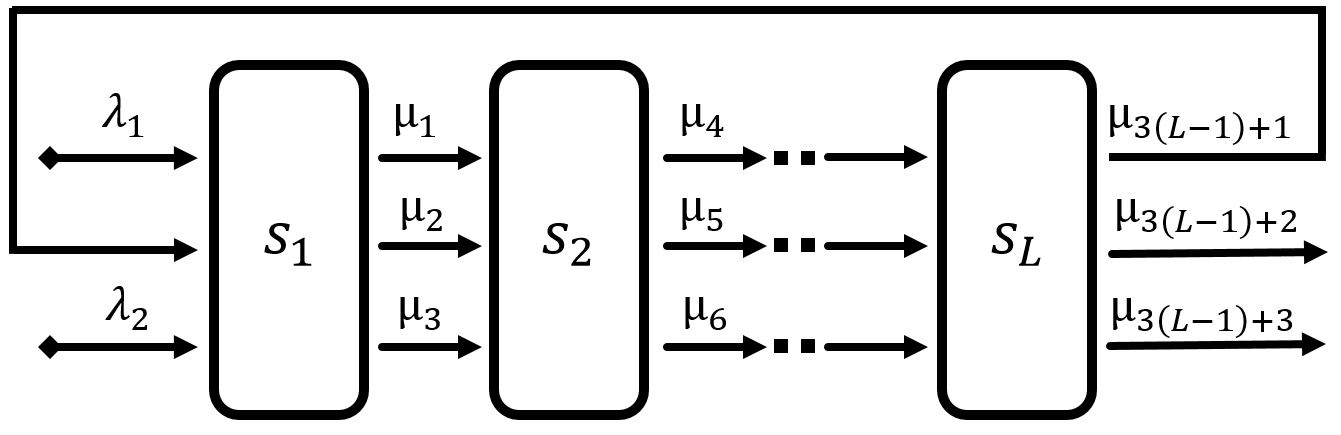
\includegraphics[width=.8\linewidth]{Paper_ext6.JPG}
\caption[]{The extended six-class network}
\label{fig1}%
\end{figure}

\begin{table}[H]
\centering%
\begin{tabular}{|c|c|c|c|c|c|}
  \hline
  % after \\: \hline or \cline{col1-col2} \cline{col3-col4} ...
  Num. of classes $3L$  & LBFS & FCFS & FP & RFP & RL\\\hline
  6 & 15.749 & 40.173 & 15.422 & 15.286 &14.180 \\\hline
  9 & 25.257 & 71.518 & 26.140 & 24.917& 23.166 \\\hline
  12  & 34.660 & 114.860 & 38.085 & 36.857& 32.420\\\hline
  15  & 45.110  & 157.556  & 45.962 & 43.628& 40.508\\\hline
  18  & 55.724 & 203.418 & 56.857  & 52.980  & 50.034\\\hline
  21  & 65.980 & 251.657 & 64.713 & 59.051 & 56.947\\
  \hline
\end{tabular}
\caption[]{Numerical results for the extended six-class network of Figure \ref{fig1}.}\label{tab6extRes}
\end{table}

\subsection{Extended re-entrant queuing network}


Another network that has been proposed in \cite{Bertsimas2015} is a reentrant line with $L$ servers. Figure \ref{fig2} displays the
topology of this queueing network. Only buffer 1 is fed by external arrivals according to a Poisson process with a rate $\lambda_1$. The network consists of $L$ services. To leave the system each job has to re-enter each server three times, thus each server processes 3 classes of jobs. The arrival rate $\lambda_1$ and all service rates of the job classes are the same as for the extended
six-class network considered in Section \ref{sec:ext}.

Learning curves showing the average number of jobs for each network are shown in Figure \ref{fig:reent_ac}.

\begin{figure}[H]
\centering%
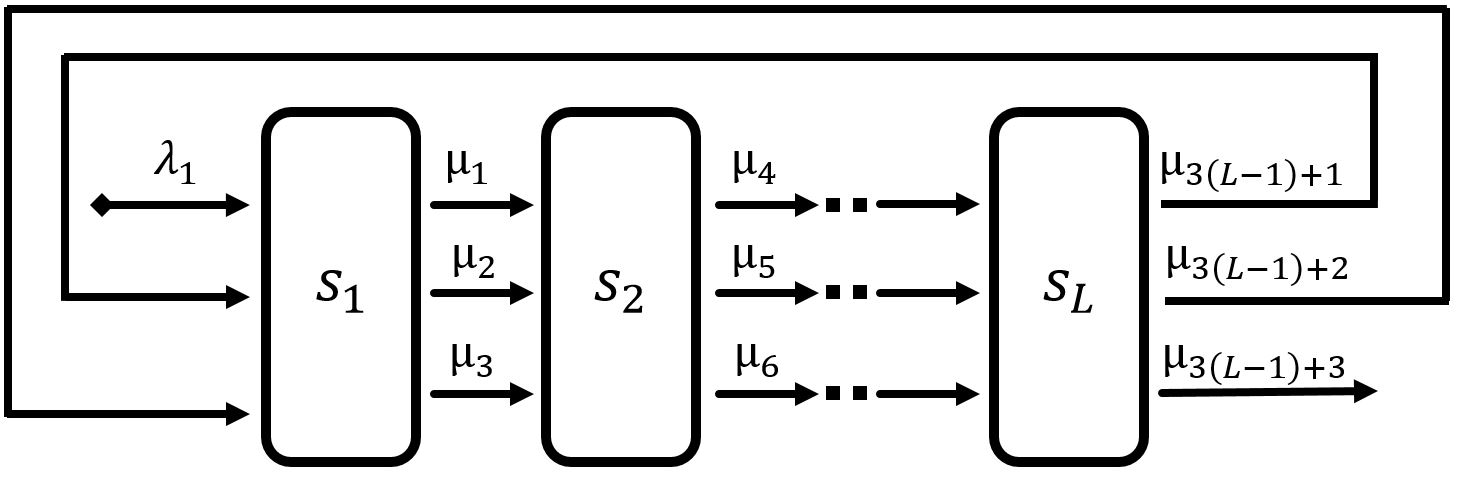
\includegraphics[width=.8\linewidth]{Paper_reentr.JPG}
\caption[]{The extended re-entrant network}
\label{fig2}%
\end{figure}

\begin{table}[H]
\centering%
\begin{tabular}{|c|c|c|c|c|c|}
  \hline
  % after \\: \hline or \cline{col1-col2} \cline{col3-col4} ...
  Num. of classes $3L$  & LBFS & FCFS & FP & RFP & RL\\\hline
  6 & 15.911 & 16.441 & 15.422 & 15.663 & 14.317\\\hline
  9 & 30.001 & 27.154 & 25.955 & 24.015& 22.359 \\\hline
  12  & 40.167 & 35.633 & 32.014 & 29.925& 28.856\\\hline
  15  & 57.056  & 47.969  & 40.113 & 36.901& 36.003\\\hline
  18  & 66.042 & 56.996 & 48.781  & 44.261  & 46.670\\\hline
  21  & 87.136 & 71.002 & 54.711 & 48.418 & 51.512\\
  \hline
\end{tabular}
\caption[]{Numerical results for the reentrant network of Figure \ref{fig2}.}\label{tabReentr}%
\end{table}





\section{Conclusion}

In this study we have presented application of
deep reinforcement learning to the scheduling problem in multiclass queuing networks.




We have  proposed a theoretically-justified modification of the Proximal Policy Optimization algorithm that can be applied in the long-run average setting.  The algorithm does not require any knowledge of  topological routing structure within the network and any information about traffic intensity. Admittedly, the learning process of the RL algorithm requires intensive simulations of many different policies that may require a generative model. The proposed approach scales well and can handle networks with multiple job classes and servers if advanced enough computational infrastructure is available.






Our numerical results show that  RL policies yield almost-optimal performance for the criss-cross network and accomplish  long-run average performance within 1\% from the optimal according to Table \ref{tab:cc}. In large networks our approach leads to effective scheduling policies that outperform or perform comparable to known alternatives. In the extended six-class queuing network RL polices  outperform  the robust fluid policies on average by more than  5\%. In the extended reentrant queuing network RL polices reach comparable performance with the robust fluid policies outperforming them on the 6-, 9-, 12-, 15- classes  networks  and performing within 5\% of
RFP on 18-, 21-classes networks. Note that displayed  performance of robust fluid policy in Table \ref{tabReentr} is the performance of the best  robust fluid policy which corresponds to the best choice of policy parameters that can be different for each network. In all our experiments we have used fixed set of hyperparameters.
Nevertheless, the results for the extended re-entrant line indicate that optimization of scheduling policies for large MQNs is a challenging problem for RL methods that use discounting to approximate the policy gradient. Designing of  a stable deep RL algorithm that does not depend on the discount factor and directly optimizes long-run average performance  is an open problem.


Based on our simulation study we  provide a recommended set of hyperparameters for the algorithm in Section \ref{sec:par}  and  neural network structures for policy parametrization and approximation of the value function in Section \ref{sec:nn}. The recommended parameters of the algorithm yield stable learning process for large range of networks from the criss-cross network to the re-entrant network with 21 job classes.


Complexity of the scheduling optimization problem highly depends not only on the network topology, but on the traffic intensity. For the small criss-cross network in low traffic regime the RL policy almost coincides with the optimal policy:  up to 99\% of actions suggested  by RL policy are optimal. While   only around 85\% of actions are optimal in the heavy traffic regime, see Figure \ref{fig:cc_opt}. Therefore, the complexity of the problem can be easily adjusted.  We believe that this feature makes multiclass queuing networks potentially  good benchmark domain to test RL methods, for example cross-task generalization (transfer learning)  \cite{Nichol2018}.



In the paper we impose classical assumptions that external arrivals are Poisson and service
times are assumed to be exponentially distributed with class-dependent rates. More realistic scheduling policy optimization problem  is to design a learning algorithm for a time-dependent distribution of inter-arrival times. We hope that the current paper a small step in this direction.




\section{Appendix}





\subsection{Maximal Stability of Random Proportional Policy}\label{sec:RP}

In this section we consider random proportional policy. 

Associated with each decision is a random proportional vector for $\gamma = (\gamma_1, ..., \gamma_J)\geq 0$ and satisfies $\sum\limits_{i\in B_l} \gamma_i =1$ and $\max\limits_{i\in B_l}\gamma_i =1$ for each server $l$.



For a job class $i\in B_l$ the fraction of server $k$ the probability to get full service capacity is proportional to population size at the decision epoch. 
\begin{align*}
\Prob(\gamma_i = 1) = \frac{x_i}{\sum\limits_{j\in B_l}}
\end{align*}


Non-negative $J-$vector $\beta$ of class-level service rates going forward from a decision time $t$, 

\begin{align}
\beta_i(t) = 
\begin{cases}
\gamma_i \text{ if }z_i(t)>0,\\
0, \text{ otherwise}
\end{cases}
\end{align}

Define a non-decreaseing $J-$dimentional process $T  = \{T(t), ~t\geq 0\}$ whose $j$th component $T_j(t)$ represents the cumulative amount of service effort devoted to jth class over the time interval $(0, t].$ It can be expressed mathematically:
\begin{align}
T_j(t):=\int\limits_0^t \beta_i(u)du,\quad \text{ for each class } j\text{ and } t\geq 0.
\end{align}


In the fluid model, for all $t\geq 0$ we have


\begin{align}\label{eq:fluid}
\dot Z(t) = \lambda - (I-P')M\beta(t)\\
C\beta(t)\leq e\\
Z(t)\geq 0\\
\beta(t)\geq 0
\end{align}


The functions $Z_i(t)$ and $T_i(t)$ are absolutely continuous, and thus, differentiable almost everywhere. The equations \ref{eq:fluid} hold for all times $t$ at which $Z_i(t)$ and $T_i(t)$ are differentiable.


For a job class $i\in B_l$ the fraction of server define ``an expected'' service allocation given queue lenghts at time $t$
  $\hat \beta_i(t) := \begin{cases} \frac{z_i(t)}{\sum\limits_{j\in B_l} z_j(t)} \end{cases}$.
  
  
  
  For each initial state $z\in \Z_+^L$ and $t > 0$, 
  
  \begin{align}
  \xi_i^z(t) := \int \limits_{0}^t ( \beta_i^z(u)  - \hat \beta_i^z(u)) du
  \end{align} 

Let us explicitely write $Z^z(t, \omega)$ for a particular sample path $\omega$ of $Z^z(t).$



\begin{lemma}
Let $\{z^r: r\geq 1\}\subset \Z_+^r$ be a sequence of initial states satisfying $|z^r|\geq r^2$ for each $r\geq 1$, then with probability 1:

\begin{align}
\lim\limits_{r\rightarrow \infty} \frac{\xi^{z^r}(|z^r, \omega|) }{|z^r|}=0
\end{align}

\begin{proof}
By Chebyshev's inequality:

\begin{align}
\Prob\left\{ \omega: \frac{|\xi_i^{z^r}(|z^r, \omega|)|}{|z^r|} >\epsilon\right\}\leq \frac{\E\left[ \xi_i^{z^r} (|z^r|) \right]^2}{\epsilon^2|z^r|^2}
\end{align}


Let $\{\tau_k\}_{k=0}^K$ are the decision epochs before time and $\tau_{K+1} = |z^r|$, where $\tau_0=0$ then 

\begin{align}
&\E\left[ \xi_i^{z^r} (|z^r|) \right]^2 = \E \left[\int\limits_0^{|z^r|} (\beta(u) - \hat\beta(u))  du  \right]^2 =  \E \left[\sum\limits_{k=0}^{K}\int\limits_{\tau_k}^{\tau_{k+1}} (\beta(u) - \hat\beta(u))  du \right   ]^2=\\
&\E\sum\limits_{k=0}^{K}   \left ( \int\limits_{\tau_k}^{\tau_{k+1}} (\beta(u) - \hat\beta(u))  du \right)^2    + 2 \sum\limits_{k<k'}^{K} \E  \left ( \int\limits_{\tau_k}^{\tau_{k+1}} (\beta(u) - \hat\beta(u))  du \right)\left ( \int\limits_{\tau_k'}^{\tau_{k'+1}} (\beta(u) - \hat\beta(u))  du \right)=\\
&  \E \sum\limits_{k=0}^{K} \left ( \int\limits_{\tau_k}^{\tau_{k+1}} (\beta(u) - \hat\beta(u))  du \right)^2  \leq \E\sum\limits_{k=0}^{K}    \left ( \int\limits_{\tau_k}^{\tau_{k+1}} 1  du \right)^2\leq \E\sum\limits_{\tau'\in \text{arrivals}}(\tau'_{k+1} - \tau'_{k})^2\leq O(|z^r|) 
\end{align}
where the second inequality follows from the fact that 

\begin{align}
&\E \sum\limits_{k<k'}^{K} \E  \left ( \int\limits_{\tau_k}^{\tau_{k+1}} (\beta(u) - \hat\beta(u))  du \right)\left ( \int\limits_{\tau_k'}^{\tau_{k'+1}} (\beta(u) - \hat\beta(u))  du \right)=\\
&\E\left[ \sum\limits_{k<k'}^{K} \E  \left ( \int\limits_{\tau_k}^{\tau_{k+1}} (\beta(u) - \hat\beta(u))  du \right) \E \left[\left ( \int\limits_{\tau_k'}^{\tau_{k'+1}} (\beta(u) - \hat\beta(u))  du \right)| Z(\tau_k')\right]\right]=0
\end{align}

Hence $\Prob\left\{ \omega: \frac{|\xi_i^{z^r}(|z^r, \omega|)|}{|z^r|} >\epsilon\right\}\leq \frac{1}{\epsilon^2 r^2}$ the lemma follows from the Borel-Cantelli lemma. 

\end{proof}

\end{lemma}





\begin{theorem}
Consider a multiclass queueing network operating under the random proportional policy. Let $\{z^r:r\geq 1\}\subset \Z^r_+$ be a sequence of initial states satisfying $|z^r|\geq r^2$ for each $r\geq 1$, and let $\Omega$ be as in Lemma \ref{lem:conv}. For each $\omega\in \Omega_1 \sup \Omega_2$, all fluid limits $(\hat D, \hat T, \hat Z)$ satisfying the following: for each packet class $i\in I$

\begin{align}
\frac{d}{dt}\hat T_i(t) = \frac{\hat Z_i(t)}{\sum\limits_{j\in B_l} \hat Z_j(t)}\text{ when }
\sum\limits_{j\in B_l} \hat Z_j(t)>0.
\end{align}



\begin{proof}

Assume that $\{z^r:r\geq 1\}\subset \Z_+^r$ is a sequence of initial states satisfying $|z^r|\geq r^2.$ Fix an $\omega \in \Omega_1\sup \Omega_2$. Let $(\hat D(\cdot), \hat T(\cdot), \hat Z(\cdot))$ be a fluid limit path. Fix a buffer $i$ and $t>0$, and let $l\in L$ be an assotiated server to buffer $i$. Assume that $\hat Z_i(t)>0.$ By the continuity of $\hat Z_i(\cdot)$, there exists a $\delta\in (0, t)$ s.t. 

\begin{align}
\epsilon:=\min\limits_{u\in [t-\delta, t+\delta]}\hat Z_i(u)>0. 
\end{align}

Thus, there exists $Z_i^{z_n}(u)\geq |z_n|\epsilon/2\geq 1$ for $u\in (|z_n|(t-\delta), |z_n|(t+\delta))$ and $n\geq L_0.$

Next,


\begin{align}
T_i^{z_r}(|z_r|u_2) - T_i^{z_r}(|z_r|u_1) = \int \limits_{|z_r|u_1}^{|z_r|u_2} ( \beta_i^z(u) du= \int \limits_{|z_r|u_1}^{|z_r|u_2}  \hat \beta_i^z(u) du+ \xi_i^{z_r} (|z_r|u_2) -  \xi_i^{z_r}(|z_r|u_1).
\end{align}



We have proved that $\lim\limits_{r\rightarrow \infty} \frac{1}{||z^r||}\left[ \xi_i^{z_r} (|z_r|u_2) -  \xi_i^{z_r}(|z_r|u_1) \right]= 0$.


Thus 

\begin{align}
\hat T_i^{z_n}(u_2) - \hat T_i^{z_n}(u_1) = \int\limits_{u_1}^{u_2} \hat \beta (\hat Z^{z_r}(u))du = \int\limits_{u_1}^{u_2}
\end{align}
\end{proof}
\end{theorem}


 





\subsection{Proofs}\label{sec:proofs}




  \begin{definition}
We denote  the discounted future state distribution starting at state $s$  by
\begin{equation}
d_\pi^s(x) = (1-\beta)\sum\limits_{t=0}^{\infty} \beta^t P_\pi(x_t = x| x_0 = s),
\end{equation}

where $P_\pi(x_t = x| x_0 = s) = P^t_\pi(x_1 = x| x_0 = s)$ is a probability od visiting state $x$ at time $t$ if we start at state $s$ and follow policy $\pi$.
\end{definition}



\begin{theorem}\label{Vnu}
\begin{equation}
\eta_\pi = (1-\beta) \E_{x\sim\mu_\pi} V^\beta_\pi(x)
\end{equation}

\begin{proof}
The proof is given in \cite[Section 10.4]{Sutton2018}.
\end{proof}
\end{theorem}


\begin{theorem}\label{thm2}
For any policies $\pi$ and $\pi'$ we have

\begin{equation}
\eta_{\pi'}-\eta_\pi  \leq  (1-\beta) \E_{x\sim\mu_\pi} \Big[V^\beta_{\pi'}(x) -V^\beta_{\pi}(x)\Big] + 2\kappa_2(S_{\pi'})||g||_2 \frac{1-\beta}{ 1 - \beta|\lambda_2(P_{\pi'})|} || D ||_1 \E_{x\sim \mu_{\pi}} D_{TV}(\pi'||\pi)[x],
\end{equation}

where $\kappa_2(S_{\pi'}) = ||S_{\pi'}||_2||S_{\pi'}^{-1}||_2$ is a spectral conditional number of the matrix  $S_{\pi'} =(s_1, s_2, .., s_n)$ where $s_i$ are right eigenvectors of $P_{\pi'}$;

 $\lambda_2(P_{\pi'})$ is a second largest eigenvalue of $P_{\pi'};$

 $\Omega_{\pi'}$ is a matrix with equal rows $\mu_{\pi'}$;

$D = (I - P_{\pi'} +\Omega_{\pi'} )^{-1} -\Omega$ is a deviation matrix of $P_{\pi'}$, $||D||_1$ is known to be finite if $P_{\pi'}$ is uniformly ergodic \cite{Kartashov1985};

$\E_{x\sim \mu_{\pi}} D_{TV}(\pi'||\pi)[x] = \frac{1}{2}\E_{x\sim \mu_{\pi}} || \pi(\cdot|x) - \pi'(\cdot|x) ||_1 =\frac{1}{2} \sum\limits_{x\in X} \mu_\pi(x) \sum\limits_{a\in A}| \pi(a|x) - \pi'(a|x)|$.
\begin{proof}

From \cite[Theorem 3.]{Baxter2001} we have the following equality:


\begin{equation}\label{eq1}
(1-\beta)  V^\beta_{\pi'} = \eta_{\pi'}e +  S(\mu_\pi') \text{diag}(0, \frac{1-\beta}{ 1 - \beta|\lambda_2(P_\pi')|},  ..., \frac{1-\beta}{ 1 - \beta|\lambda_n(P_\pi')|})S^{-1}(\mu_\pi')g,
\end{equation}
where $V_{\pi'}^\beta$ is a vector form of $[V^\beta_{\pi'}(x)]_{x\in X}$, $e = (1, 1, ..., 1)^T$
$\lambda_1(P_\pi') =  1>  |\lambda_2(P_\pi')|\geq\lambda_n(P_\pi')$ are eigenvalues of $P_\pi'$ (we assume that $P_\pi'$ has n district eigenvalues.)


Now we consider a difference between expectation of equation \ref{eq1} taken over stationary distribution $\mu_\pi$ and expectation of this equation taken over $\mu_{\pi'}.$
\begin{equation}
(1-\beta) \E_{x\sim\mu_\pi} V_{\pi'}(x) = \eta_\pi' + (\mu_\pi - \mu_\pi')^T S(\mu_\pi') \text{diag}(0, \frac{1-\beta}{ 1 - \beta|\lambda_2(\mu_\pi')|},  ..., \frac{1-\beta}{ 1 - \beta|\lambda_n(\mu_\pi')|})S^{-1}(\mu_\pi')g,
\end{equation}

where we use the fact from Theorem \ref{Vnu} that $\E_{x\sim\mu_\pi} V_{\pi}(x) = \eta_\pi$.

The last term can be bounded using Cauchy-Schwarz inequality:


\begin{align}
\Big|(\mu_\pi - \mu_\pi')^T S(\mu_\pi') \text{diag}(0, \frac{1-\beta}{ 1 - \beta|\lambda_2(\mu_\pi')|},  ..., \frac{1-\beta}{ 1 - \beta|\lambda_n(\mu_\pi')|})S^{-1}(\mu_\pi')g\Big|\geq&\\
- || \mu_\pi - \mu_\pi'||_2||S(\mu_\pi')\Big|\Big|\text{diag}(0, \frac{1-\beta}{ 1 - \beta|\lambda_2(\mu_\pi')|},  ..., \frac{1-\beta}{ 1 - \beta|\lambda_n(\mu_\pi')|})\Big|\Big|_2||S^{-1}(\mu_\pi')g||_2\geq&\\
\kappa_2(S)||g||_2 \frac{1-\beta}{ 1 - \beta|\lambda_2(\mu_\pi')|} ||\mu_{\pi'} - \mu_\pi||_2,
\end{align}
where $||diag(d_1, d_2, .., d_n)||_2\leq \max_i d_i$ and $\kappa_2(S) = ||S||_2||S^{-1}||_2$.


We can get a bound on the difference between stationary distributions :
\begin{equation}
|| \mu_{\pi'} - \mu_\pi||_2\leq  || \mu_{\pi'} - \mu_\pi||_1 \leq ||\mu_\pi(P_{\pi'} - P_{\pi})||_1||D_{\pi'}||_1\leq 2\E_{x\sim \mu_{\pi'}} D_{TV}(\pi'||\pi)[x]||D_{\pi'}||_1,
\end{equation}
where the second inequality follows from equality $\mu_\pi - \mu_\pi' = \mu_\pi(P_\pi - P_{\pi'})D$, see \cite[Section 2]{Liu2012}   and the last inequality follows from \cite[Lemma 3]{Achiam2017}.
\end{proof}

\end{theorem}




\begin{theorem}\label{thm:distr}
\begin{equation}
\underset{s\sim\mu_\pi}{\E}\left[\underset{\substack{x\sim d_\pi(s)\\a\sim\pi(\cdot|x)  \\  x'\sim P(\cdot|x, a)}  }{\E}  f(x, a, x') \right]= \underset{\substack{x\sim \mu_\pi\\a\sim\pi(\cdot|x)  \\  x'\sim P(\cdot|x, a)}  }{\E} f(x,a , x')
\end{equation}

\begin{proof}

Consider the same MDP problem but with cost-to-go function $f(x) = \underset{\substack{a\sim\pi(\cdot|x)  \\  x'\sim P(\cdot|x, a)}  }{\E}  f(x, a, x') $. Then $\frac{1}{1-\beta}E_{x\sim d_\pi(s)} f(x) $ is the infinite horizon discounted total costs at state $s$ of policy $\pi$. The result follows from Theorem \ref{Vnu}.

\end{proof}
\end{theorem}





\begin{theorem}
For any function $f:X\rightarrow \R $ and any policies $\pi'$ and $\pi$, define


\begin{itemize}
  \item \begin{equation}
\delta_f(s, a, x') = g(x) +\beta f(x') - f(x)
\end{equation}
  \item its max-bound:
\begin{equation}
\epsilon_f^\pi = \max\limits_{x\in X} \underset{\substack{ a\sim \pi(\cdot|x)\\x'\sim P(\cdot|x, a)}}{\E}[\delta_f(x, a, x')]
\end{equation}

\item For transition matrix $P_{\pi'}$ and discount factor $\beta$ we define
\begin{equation}
 a_{\pi'} = \kappa_2(S_{\pi'})\frac{1-\beta}{ 1 - \beta|\lambda_2(P_{\pi'})|} || D_{\pi'} ||_1,
  \end{equation}
where

\begin{itemize}
  \item[*]  $\kappa_2(S_{\pi'}) = ||S_{\pi'}||_2||S_{\pi'}^{-1}||_2$ is a spectral conditional number of the matrix  $S_{\pi'} =(s_1, s_2, .., s_n)$ where $s_i$ are right eigenvectors of $P_{\pi'}$;
  \item[*] $\lambda_2(P_{\pi'})$ is a second largest eigenvalue of $P_{\pi'};$
  \item[*] $\Omega_{\pi'}$ is a matrix with equal rows $\mu_{\pi'}$;
  \item[*] $D = (I - P_{\pi'} +\Omega_{\pi'} )^{-1} -\Omega$ is a deviation matrix of $P_{\pi'}$, $||D||_1$ is known to be finite if $P_{\pi'}$ is uniformly ergodic \cite{Kartashov1985};
\end{itemize}









  \item \begin{equation}
L_{\pi,f}(\pi') =  \underset{\substack{ x\sim \mu_\pi\\ a\sim \pi(\cdot|x)\\x'\sim P(\cdot|x, a)}}{\E}\left[\left( \frac{\pi'(a| x)}{\pi(a|x)}-1 \right)\delta_f(x, a, x') \right]
\end{equation}
  \item $D_{\pi, f}^{\pm} (\pi') = L_{\pi,f}(\pi')\pm 2\left(\frac{\beta}{1-\beta}\epsilon_f^{\pi'} +  ||g||_2 a_{\pi'}\right) \E_{x\sim \mu_\pi}[D_{TV}(\pi'||\pi)[x]]$,

  where $\E_{x\sim \mu_{\pi}} D_{TV}(\pi'||\pi)[x] = \frac{1}{2}\E_{x\sim \mu_{\pi}} || \pi(\cdot|x) - \pi'(\cdot|x) ||_1 =\frac{1}{2} \sum\limits_{x\in X} \mu_\pi(x) \sum\limits_{a\in A}| \pi(a|x) - \pi'(a|x)|$.
\end{itemize}


The following bound for long-run average cost holds:

\begin{equation}\label{eq_main}
D_{\pi, f}^{-} (\pi')\geq \eta_{\pi'} - \eta_\pi\geq D_{\pi, f}^{+} (\pi')
\end{equation}

In particular, if we take $f(x) = V_\pi(x)$ we get $\delta_V(x, a, x') = A_\pi(x, a)$ and


\begin{equation}
 \eta_{\pi'} - \eta_\pi\leq \underset{\substack{ x\sim \mu_\pi\\ a\sim \pi(\cdot|x)}}{\E}\left[\left( \frac{\pi'(a| x)}{\pi(a|x)}-1 \right)A_\pi(x, a) \right] + 2\left(\frac{\beta}{1-\beta}\epsilon_V^{\pi'} +  ||g||_2 a_{\pi'}\right) \E_{x\sim \mu_\pi}[D_{TV}(\pi'||\pi)[x]]
\end{equation}
\begin{proof}
Consider inequality \ref{eqV_V2} from Lemma \ref{lem1} and show one side of inequality \ref{eq_main}. Starting from inequality \ref{eqV_V} one can show opposite side  of inequality \ref{eq_main}.

Assuming that initial states $s$ are sampled from a stationary distribution of policy $\pi$ we get:

\begin{align*}
&(1-\beta)\E_{s\sim \mu_\pi}\left[ V_{\pi'}(s) - V_\pi(s)\right] \leq\\& \E_{s\sim \mu_\pi}\left[\underset{\substack{ x\sim d^s_\pi\\ a\sim \pi(\cdot|x)\\x'\sim P(\cdot|x, a)}}{\E}\left[\left( \frac{\pi'(a| x)}{\pi(a|x)}-1 \right)\delta_f(x, a, x') \right]  + \frac{2\beta}{1- \beta}||\delta_{f,\pi'}^s ||_\infty \E_{x\sim d^s_\pi} [D_{TV}(\pi'||\pi)[x]] \right]
\end{align*}



Then from Theorem \ref{thm:distr} we have:
\begin{itemize}
  \item $\E_{s\sim \mu_\pi}\left[\underset{\substack{ x\sim d^s_\pi\\ a\sim \pi(\cdot|x)\\x'\sim P(\cdot|x, a)}}{\E}\left[\left( \frac{\pi'(a| x)}{\pi(a|x)}-1 \right)\delta_f(x, a, x') \right]\right] = \underset{\substack{ x\sim \mu_\pi\\ a\sim \pi(\cdot|x)\\x'\sim P(\cdot|x, a)}}{\E}\left[\left( \frac{\pi'(a| x)}{\pi(a|x)}-1 \right)\delta_f(x, a, x') \right]$
  \item $\E_{s\sim \mu_\pi}\left[ \frac{2\beta}{1- \beta}||\delta_{f,\pi'}^s ||_\infty \E_{x\sim d^s_\pi} [D_{TV}(\pi'||\pi)[x]] \right] =  \frac{2\beta}{1- \beta}||\delta_{f,\pi'} ||_\infty \E_{x\sim \mu_\pi} [D_{TV}(\pi'||\pi)[x]] $
\end{itemize}
Hence

\begin{align*}
&(1-\beta)\E_{s\sim \mu_\pi}\left[ V_{\pi'}(s) - V_\pi(s)\right] \leq \\& \underset{\substack{ x\sim \mu_\pi\\ a\sim \pi(\cdot|x)\\x'\sim P(\cdot|x, a)}}{\E}\left[\left( \frac{\pi'(a| x)}{\pi(a|x)}-1 \right)\delta_f(x, a, x') \right]  + \frac{2\beta}{1- \beta}||\delta_{f,\pi'} ||_\infty \E_{x\sim \mu_\pi} [D_{TV}(\pi'||\pi)[x]]
\end{align*}


Combining the last equation with Theorem \ref{thm2} we get



\begin{align}
&\eta_{\pi'}-\eta_\pi  \leq  (1-\beta) \E_{x\sim\mu_\pi} \Big[V_{\pi'}(x) -V_{\pi}(x)\Big] + 2a_{\pi'}||g||_2 \E_{x\sim \mu_{\pi}} D_{TV}(\pi'||\pi)[x]\leq\\
&\underset{\substack{ x\sim \mu_\pi\\ a\sim \pi(\cdot|x)\\x'\sim P(\cdot|x, a)}}{\E}\left[\left( \frac{\pi'(a| x)}{\pi(a|x)}-1 \right)\delta_f(x, a, x') \right]  + \frac{2\beta}{1- \beta}||\delta_{f,\pi'} ||_\infty \E_{x\sim \mu_\pi} [D_{TV}(\pi'||\pi)[x]] + 2a_{\pi'}||g||_2 \E_{x\sim \mu_{\pi}} D_{TV}(\pi'||\pi)[x]
\end{align}




\end{proof}
\end{theorem}

\begin{lemma}\label{lem1}

\begin{equation}\label{eqV_V}
 V_{\pi'}(s) - V_\pi(s) \geq \frac{1}{1 - \beta} \left( \underset{\substack{ x\sim d^s_\pi\\ a\sim \pi(\cdot|x)\\x'\sim P(\cdot|x, a)}}{\E}\left[\left( \frac{\pi'(a| x)}{\pi(a|x)}-1 \right)\delta_f(x, a, x') \right]  - \frac{2\beta}{1- \beta}||\delta_{f,\pi'}^s ||_\infty \E_{x\sim d^s_\pi} [D_{TV}(\pi'||\pi)[x]] \right)
\end{equation}

\begin{equation}\label{eqV_V2}
V_{\pi'}(s) - V_\pi(s) \leq  \frac{1}{1 - \beta} \left( \underset{\substack{ x\sim d^s_\pi\\ a\sim \pi(\cdot|x)\\x'\sim P(\cdot|x, a)}}{\E}\left[\left( \frac{\pi'(a| x)}{\pi(a|x)}-1 \right)\delta_f(x, a, x') \right]  + \frac{2\beta}{1- \beta}||\delta_{f,\pi'}^s ||_\infty \E_{x\sim d^s_\pi} [D_{TV}(\pi'||\pi)[x]] \right)
\end{equation}




\begin{proof}

See Lemma 2 and Lemma 3 in \cite{Achiam2017}. Note that all expectations are taken w.r.t.  the discounted future state distribution $d_\pi^s(\cdot)$ starting at state $s$.
\end{proof}
\end{lemma}
\subsection{Neural Network structure}\label{sec:nn}







In the experiments we parameterized the RL policy with a neural network. The policy neural network $\pi_\theta(a|x)$ uses the system state $x$ as an input and deterministically maps it to a distribution over action space. Then we can sample an action for state $x$ according to the likelihood of each action.



To represent the policy we use a fully-connected multilayer perceptron (MLP) (except the output layer) with three hidden layers and tanh activation functions. The input layer has $J$ units corresponding to each job class, the first hidden layer consists of $10\times J$ units, the third layer has $10\times L$, where $L$ is  number of services in the queueing system. Number of units in the  second layer is a geometric mean of units in the first and third layers, that is $10\times \sqrt{LJ}$.


For the last output layer we use a factored action space, where each factor corresponds to a server and is parameterized as a categorical distribution.
We represent the output action of $\pi_\theta(a|x)$ as a tuple $(a_1, a_2, . . . , a_L)$, where $a_l\in B_l$ represents an action (priority class) for $l$th server.
Each of these components is assumed to have a categorical distribution which is specified by a probability vector $\varsigma_l = [p_j^l: j\in B_l]$, where $p_j^l$ is a probability of giving priority to $j$th class in the server $l$. In the neural network each components of $\varsigma = [\varsigma_1, ..., \varsigma_L]$ computed applying the softmax operator to the third layer yielding normalized probabilities for each factor.


To represent the value function we use a fully-connected MLP with three hidden layers and tanh activation functions. The input layer is composed of $J$ units corresponding to each job class, the first hidden layer formed of $10\times J$ units, the third layer has $10$ units. The number of units in the  second layer is $10\times \sqrt{J}$. The output layer contains one unit with a linear activation function.

\subsection{Experiment Parameters}\label{sec:par}
In this section we explore learning process of the RL algorithm under different hyperparaments settings. We chose a computationally cheap benchmark, namely the criss-cross network from Figure \ref{fig:cc} under the B.H. load condition. In each experiment we vary only one or two parameters and the rest parameters  are fixed to the values in the last column of Table \ref{tab:par}. We note that we use since the


\begin{table}[!ht]
\centering%
\begin{tabular}{|c|c|c|}
  \hline
  % after \\: \hline or \cline{col1-col2} \cline{col3-col4} ...
  Parameter  & Value\\\hline
  Clipping parameter $(\epsilon)$ & $0.2\times \alpha$ \\
  Horizon $(T)$ & 20,000 \\
  Num. of episodes/actors $(N)$  & 50 \\
  Adam stepsize for policy NN& $5\cdot 10^{-4}\times \max[ \alpha,0.1]  $   \\
  Adam stepsize for value NN& $2.5\cdot 10^{-4}  $ \\
  Discount factor $(\beta)$  & 0.995  \\
  GAE parameter $(\lambda)$  & 0.97 \\
  Num. of epochs $(K)$& 3\\
  Minibatch size & 256\\
  Skipped decision epochs & $0$ for Table \ref{tab:cc}; $3$ for the rest experiments\\
  Routine to choose int. states & Algorithm \ref{alg1}\\
  Bound for a sampled initial state $(\Lambda)$ & 300
\end{tabular}
\caption[]{Values of hyperparameters used in the experiments. Parameter $\alpha$ is linearly annealed from $1$ to $0$ over the course of learning.}\label{tab:par}
\end{table}

First we check dependency on clipping parameter. We have tested three options $\epsilon = \{0.1,0.2, 0.3\}$ that had been proposed in \cite{Schulman2017}. We have not identified any significant affect of the clipping parameter on learning and use $\epsilon = 0.2$ for the rest experiments.






   \begin{figure}[!ht]
     \subfloat[average cost\label{subfig-1:clip1}]{%
       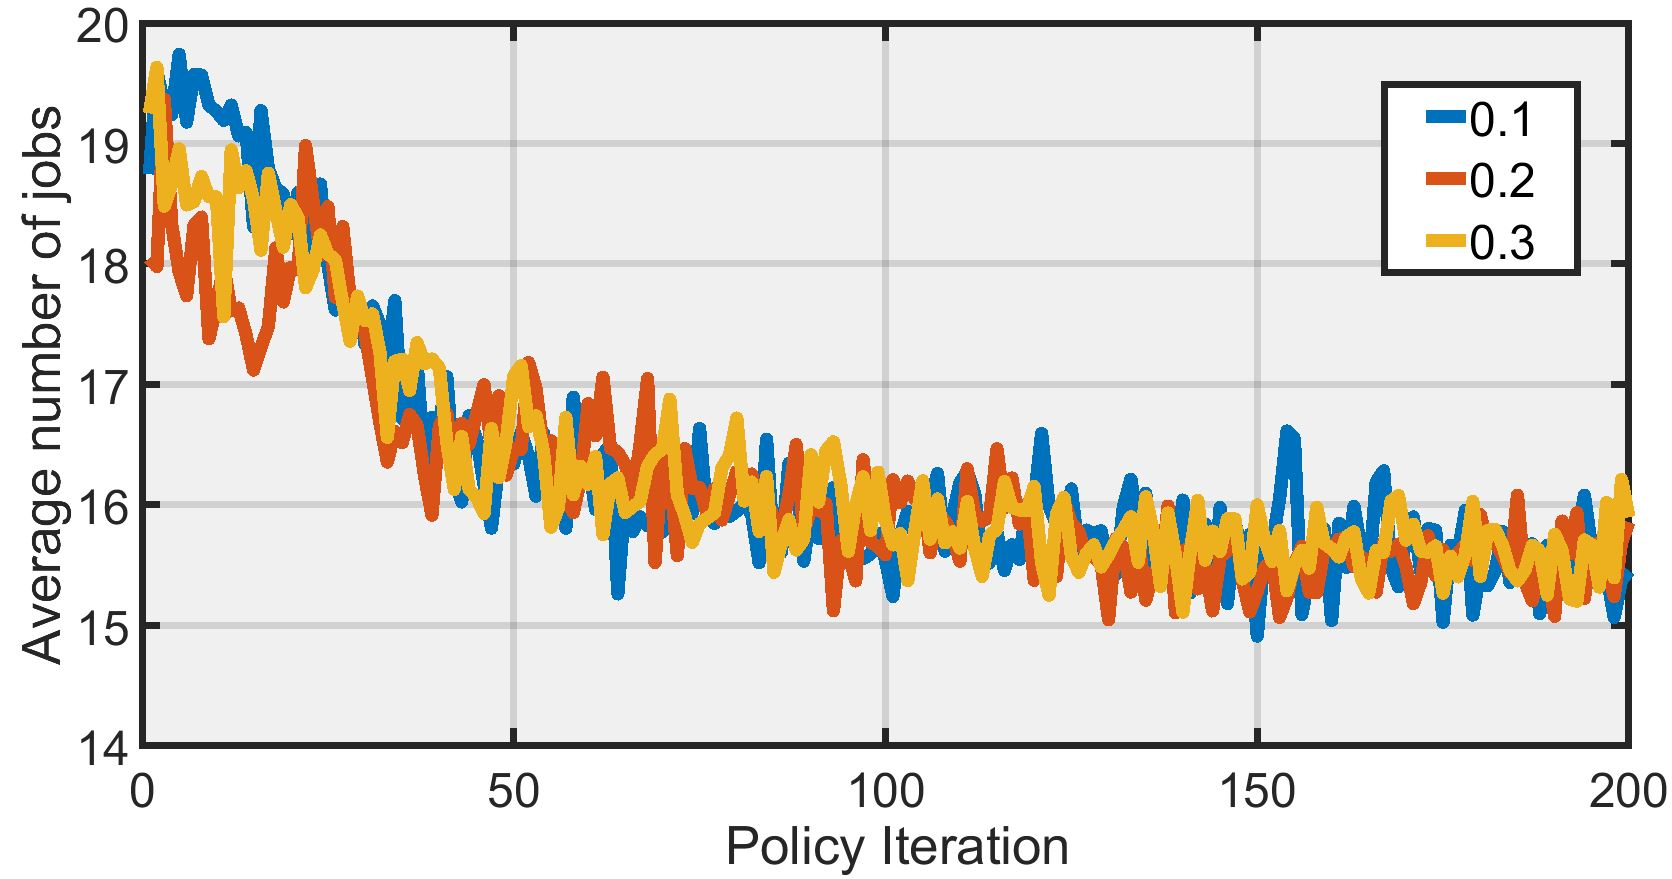
\includegraphics[width=0.45\textwidth, height=0.25\textwidth ]{Paper_clip}
     }
     \hfill
     \subfloat[Percentage of optimal actions \label{subfig-2:clip2}]{%
       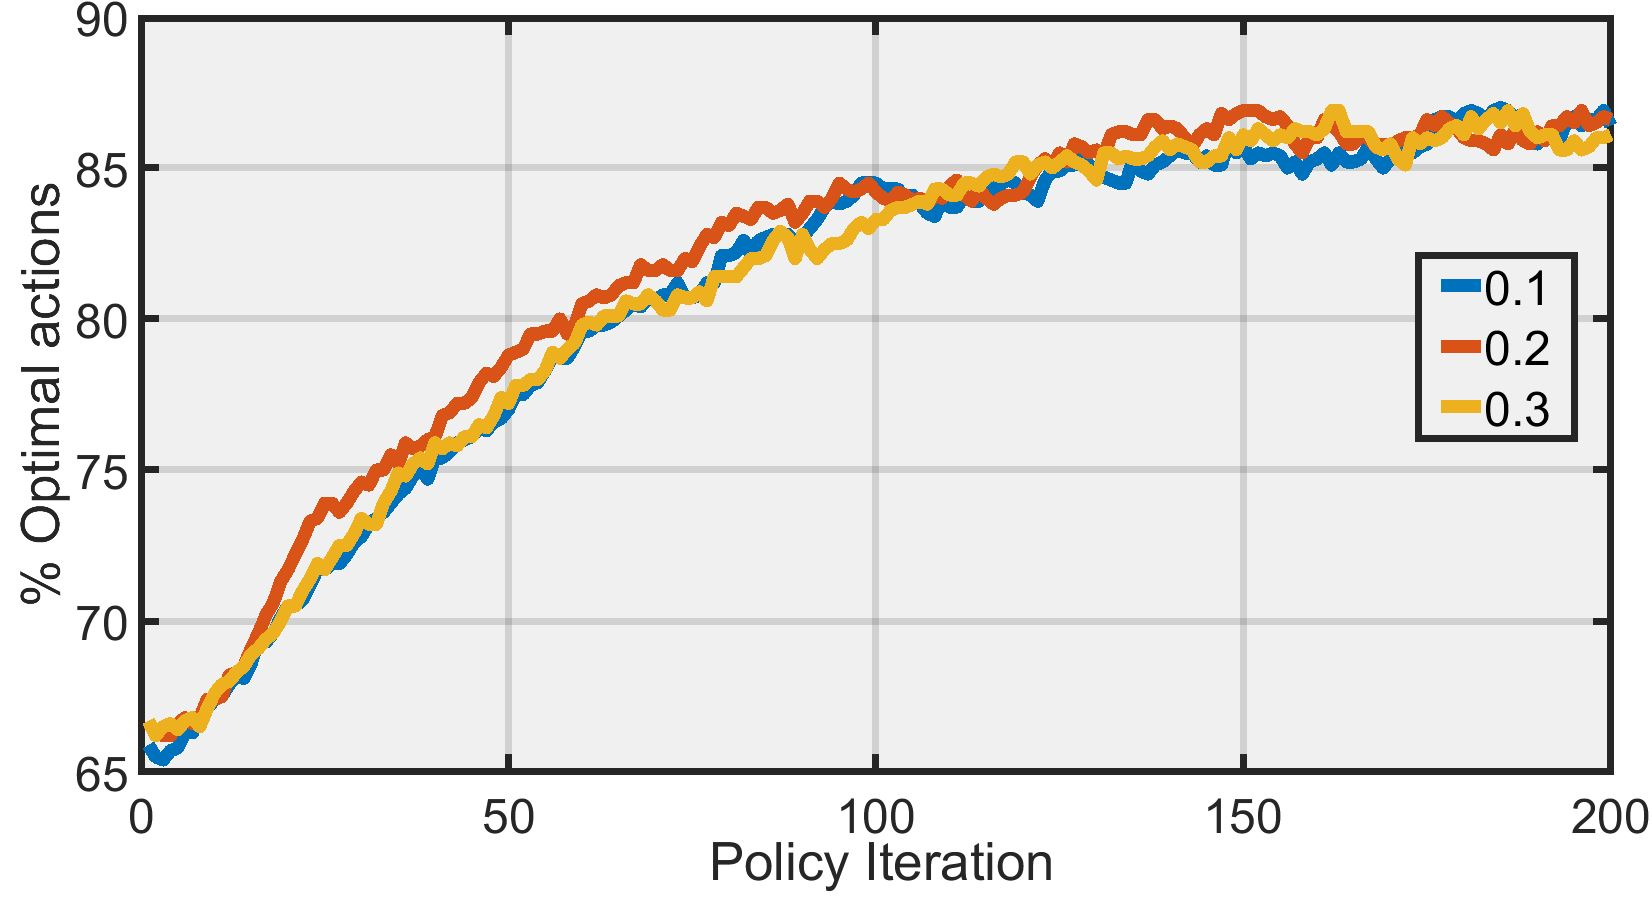
\includegraphics[width=0.45\textwidth, height=0.25\textwidth ]{Paper_clip_opt}
     }
     \caption{ Varying the clipping parameter within $\epsilon = \{0.1, 0.2, 0.3\}$ does not have  significant effect on learning.}
     \label{fig:clip}
   \end{figure}




Now we test dependency on number of episodes $E$ and their duration $T$. In Figure \ref{subfig:TE1} we fix number of episodes/actors to $N=25$ and test how the learning process depends on an episode horizon $T$. We observe that increasing horizon more than $T=40000$ does not yield further improvement. Next we fix total sample size to $T\times N = 10^9$ and examine the trade-off between number of episodes $N$ and an episode duration $T$.    In Figure \ref{subfig:TE2} we show learning curves for three sets of parameters $\{(T=10000, N=100), (T=20000, N=50), (T=40000, N=25)\}$. We observe that $ T=20000$ and $N=50$ is the best combination.


   \begin{figure}[!ht]
     \subfloat[  Results for different values of $T$ if number of actors is fixed $N=25$. \label{subfig:TE1}]{%
       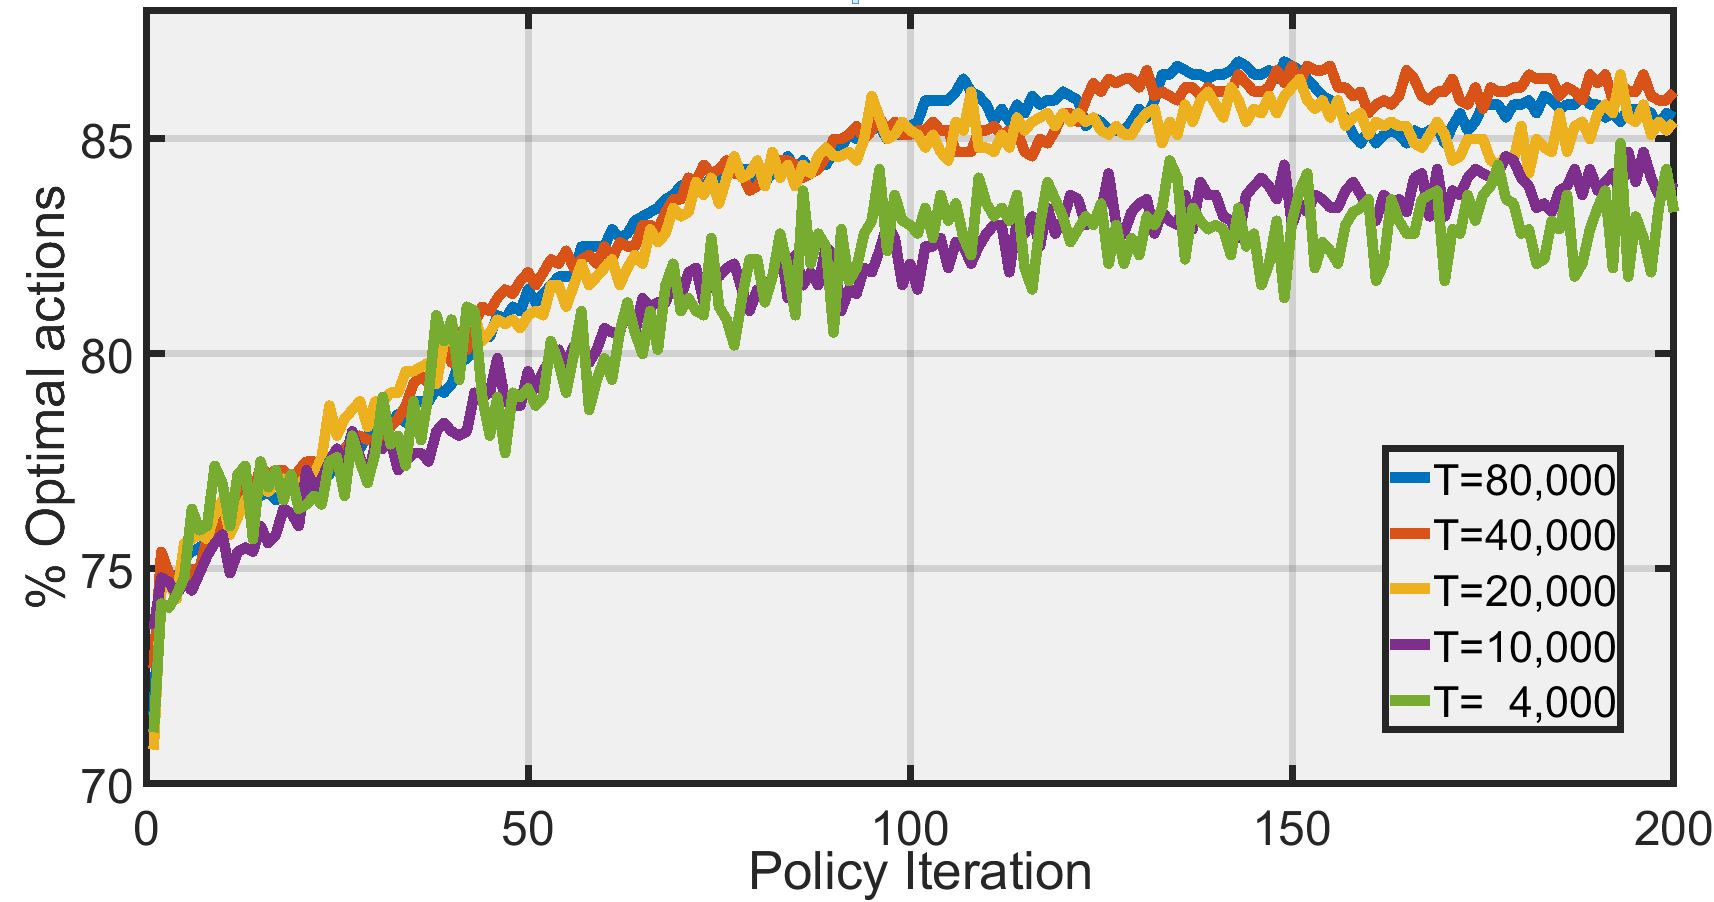
\includegraphics[width=0.45\textwidth, height=0.25\textwidth ]{Paper_SC_opt}
     }
     \hfill
     \subfloat[Trade-off between the number of actors $N$ and horizon length $T$.\label{subfig:TE2}]{%
       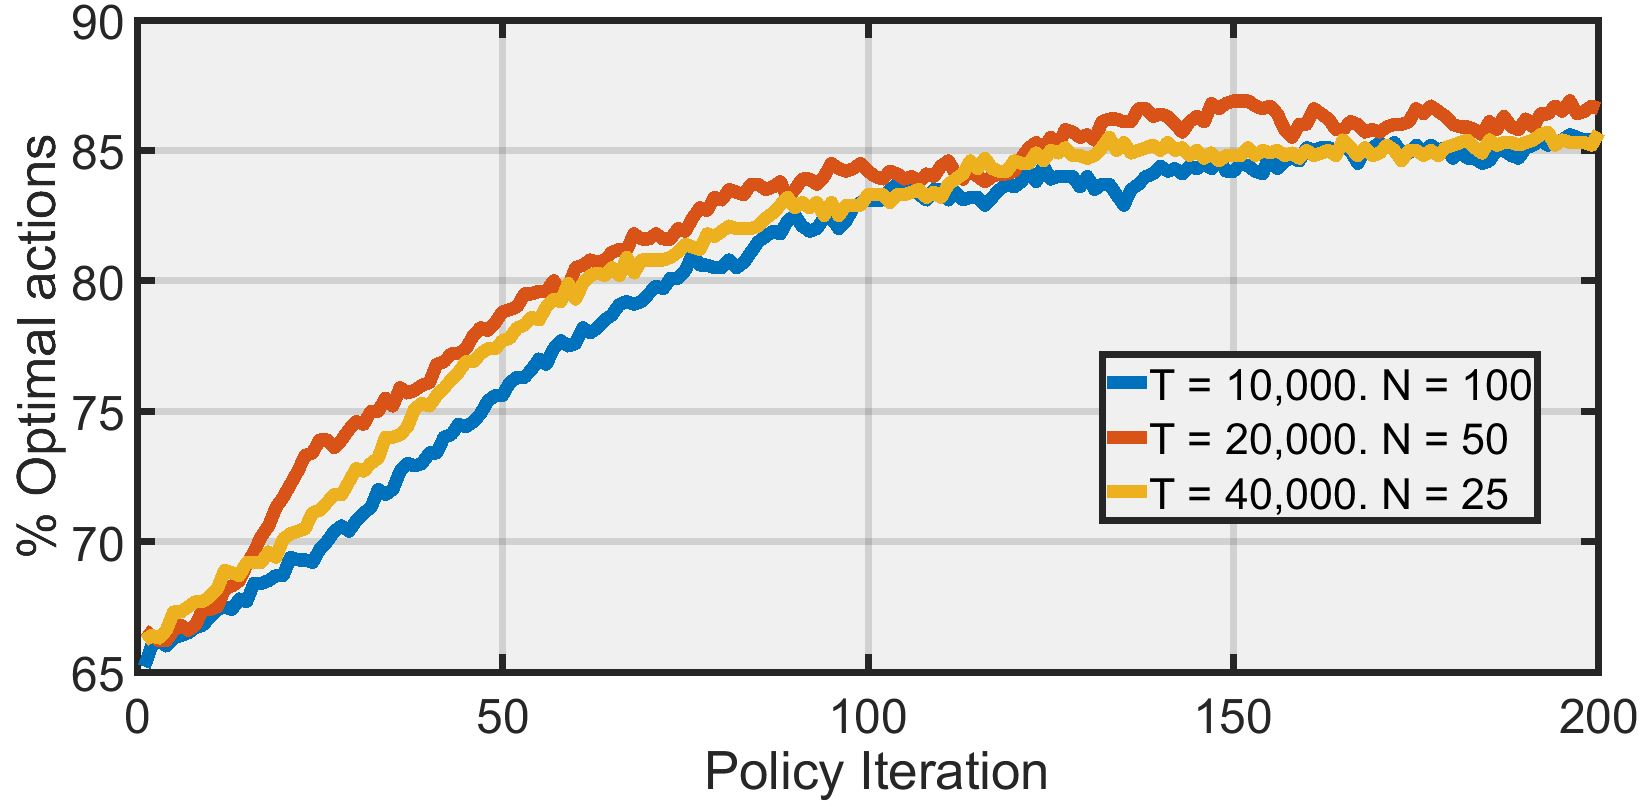
\includegraphics[width=0.45\textwidth, height=0.25\textwidth ]{PaperTE}
     }
     \caption{Effect of episode duration $T$ and number of actors $N$ on the learning process. }
     \label{fig:TE}
   \end{figure}



Another important parameter is discount factor $\beta$. We examine a discount factor jointly with GAE parameter $\lambda.$ In our tests parameters $\beta = 0.995$ and $\lambda = 0.97$ yield the best result.


\begin{figure}[H]
\centering%
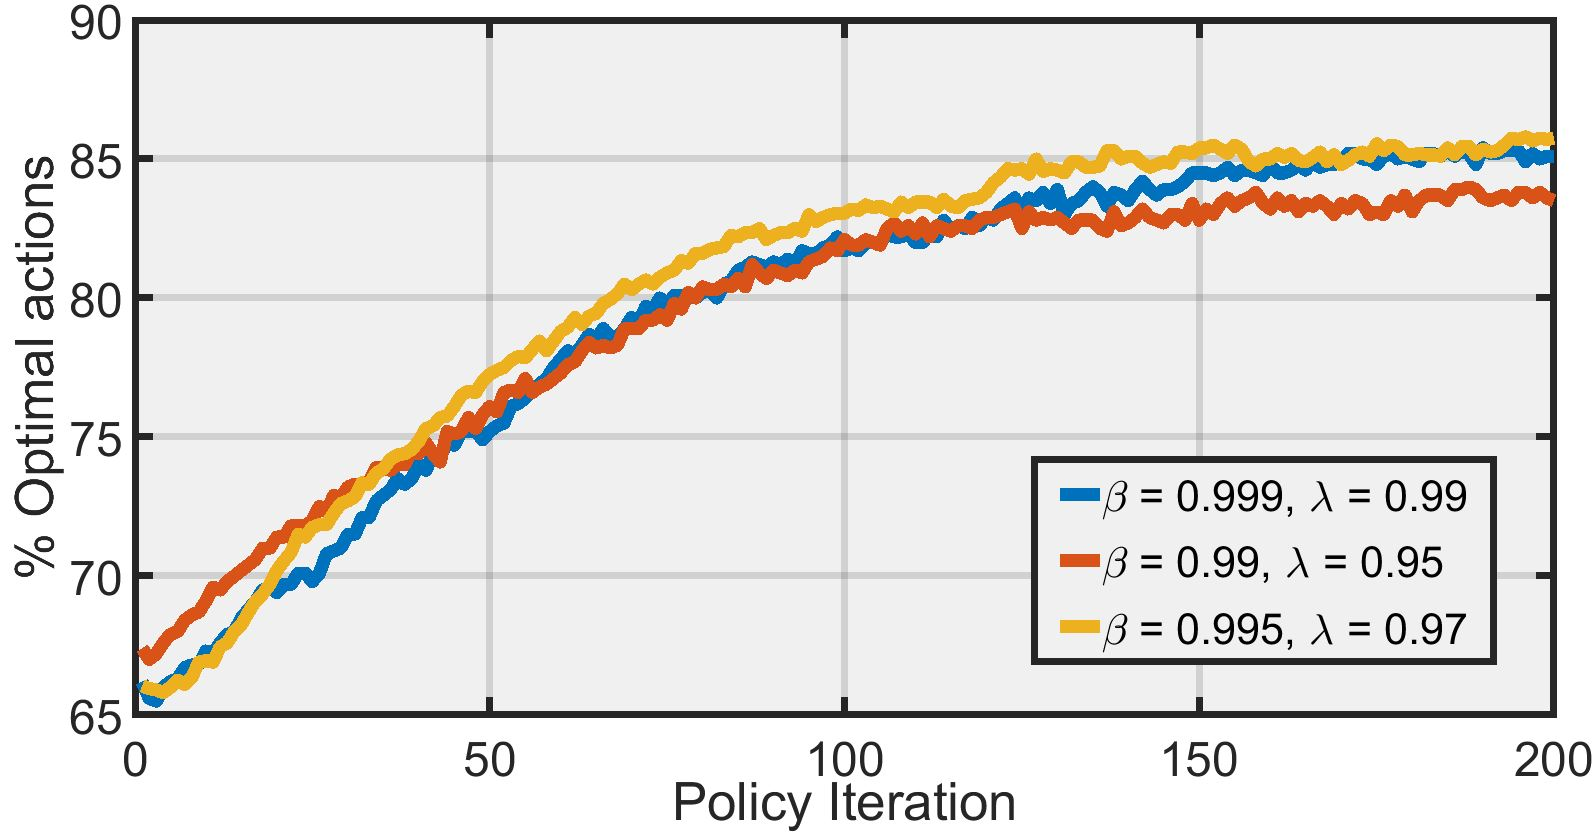
\includegraphics[width=0.55\textwidth, height=0.30\textwidth]{Paper_beta.JPG}
\caption[]{Effect of discount factor and GAE parameter.  }
\label{fig:beta}%
\end{figure}


\subsection{Learning Curves}








  \begin{figure}[H]
     \subfloat[Balanced heavy (BH) traffic\label{subfig-1:BH}]{%
       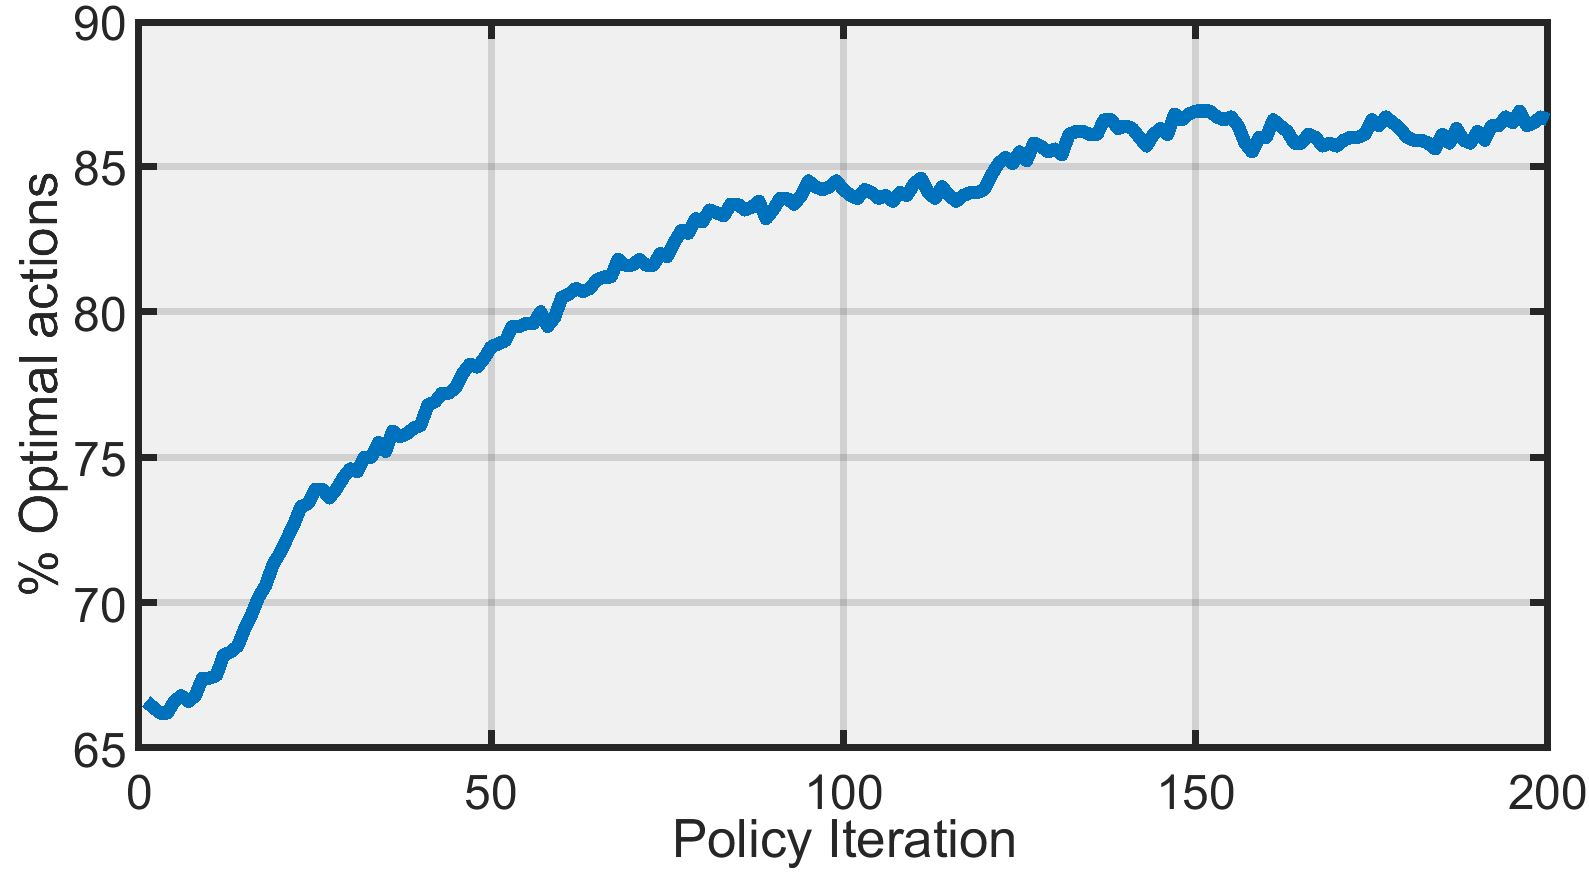
\includegraphics[ height=0.2\textwidth, width=0.35\textwidth]{Paper_BH_opt}
     }
     \subfloat[Balanced medium (BM) traffic\label{subfig-3:BM}]{%
       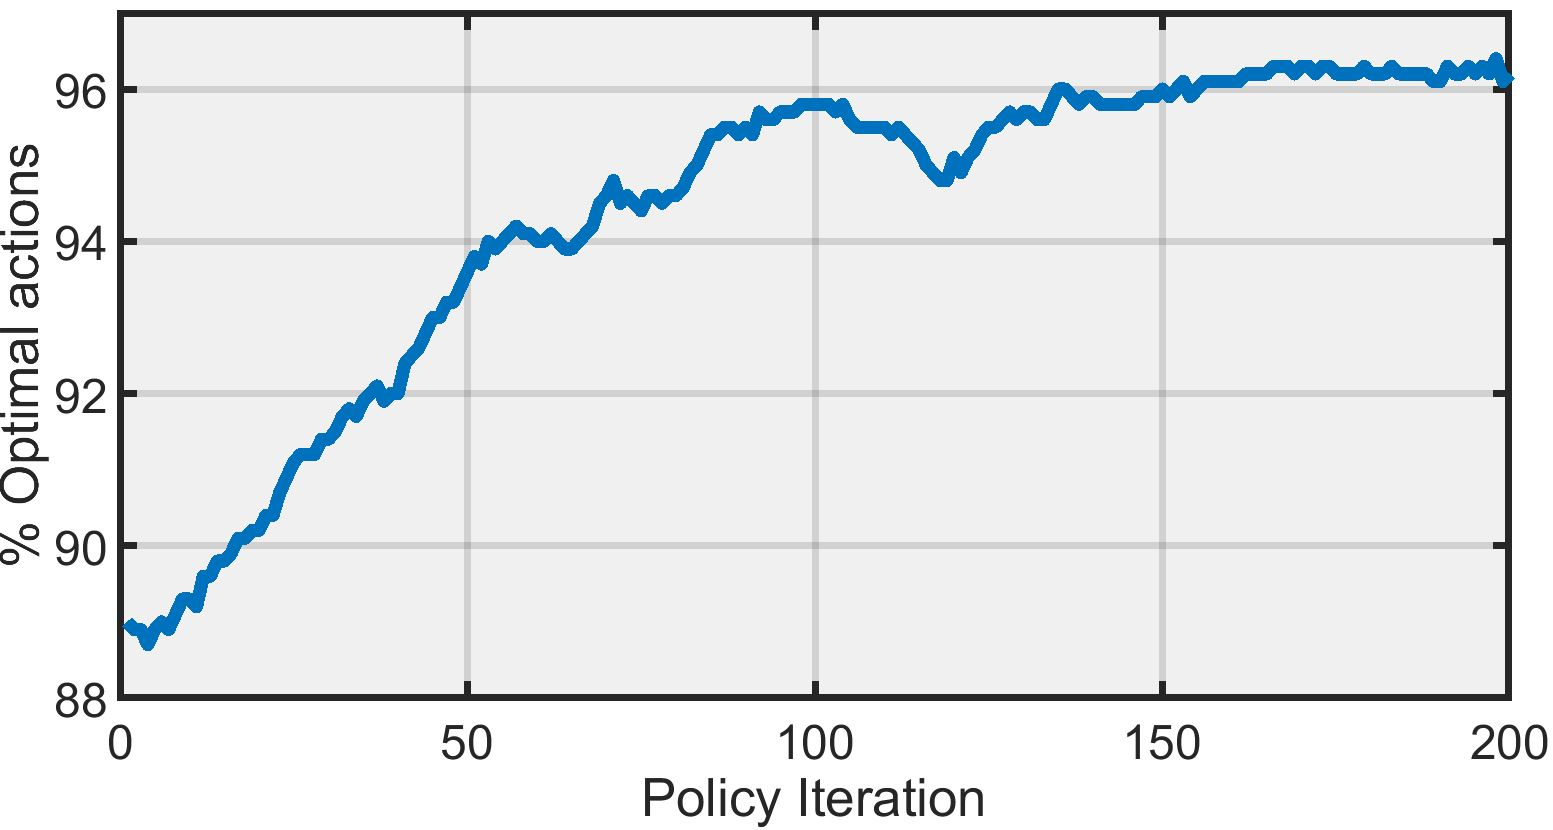
\includegraphics[  height=0.2\textwidth, width=0.35\textwidth]{Paper_BM_opt}
     } 
     \subfloat[Balanced low (BL) traffic\label{subfig-5:BL}]{%
       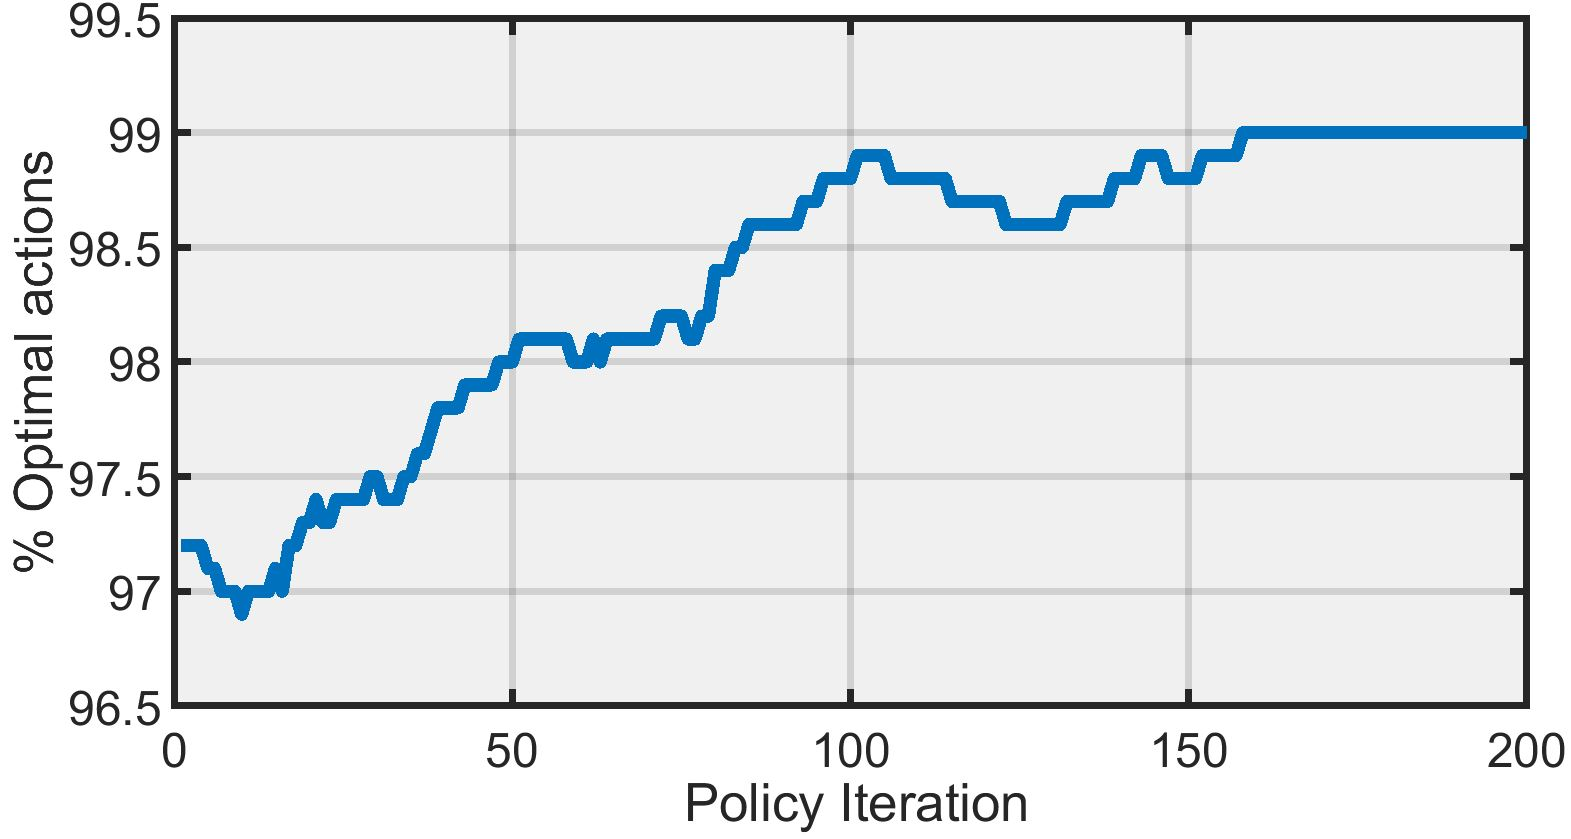
\includegraphics[  height=0.2\textwidth, width=0.35\textwidth]{Paper_BL_opt}
     }\\
     \subfloat[Imbalanced heavy (IH) traffic \label{subfig-2:IH}]{%
       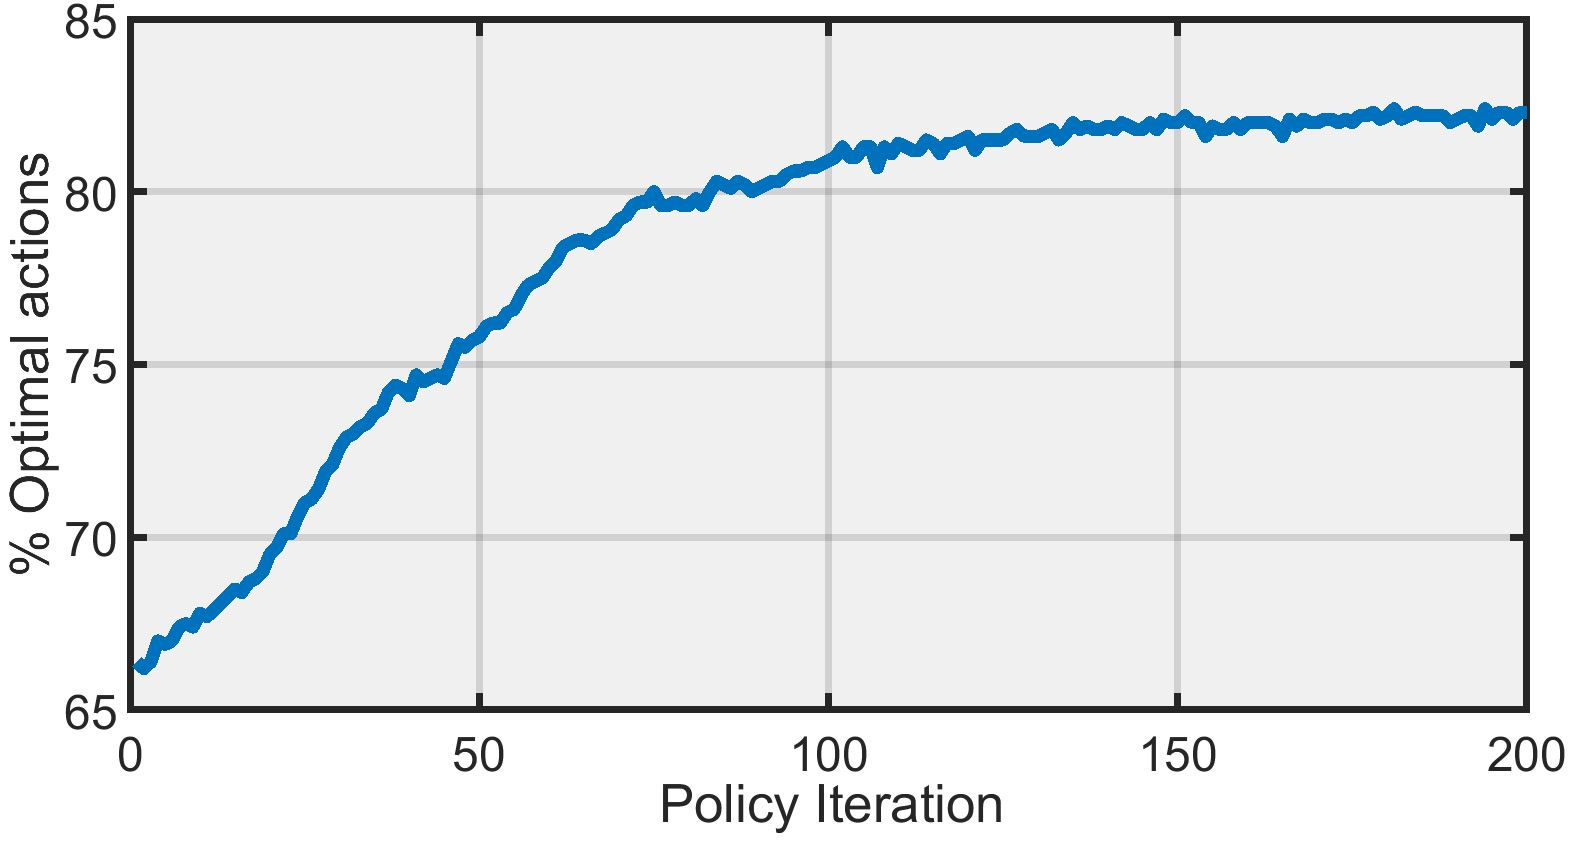
\includegraphics[ height=0.2\textwidth, width=0.35\textwidth]{Paper_IH_opt}
     }
     \subfloat[Imbalanced medium (IM) traffic \label{subfig-4:IM}]{%
       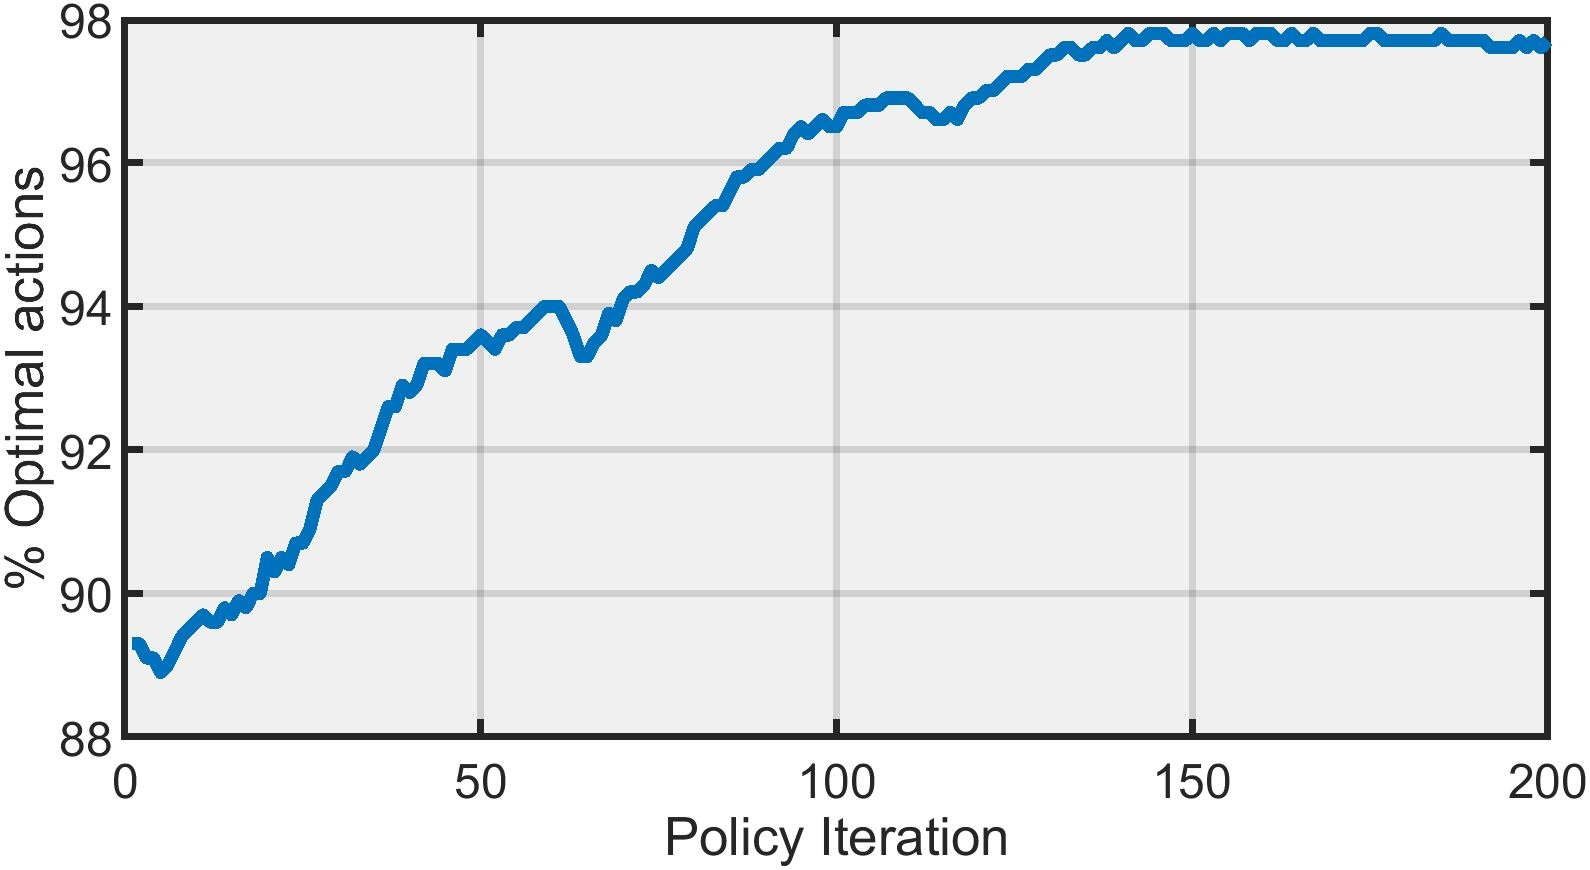
\includegraphics[ height=0.2\textwidth, width=0.35\textwidth]{Paper_IM_opt}
     }
     \subfloat[Imbalanced low (IL) traffic \label{subfig-6:IL}]{%
       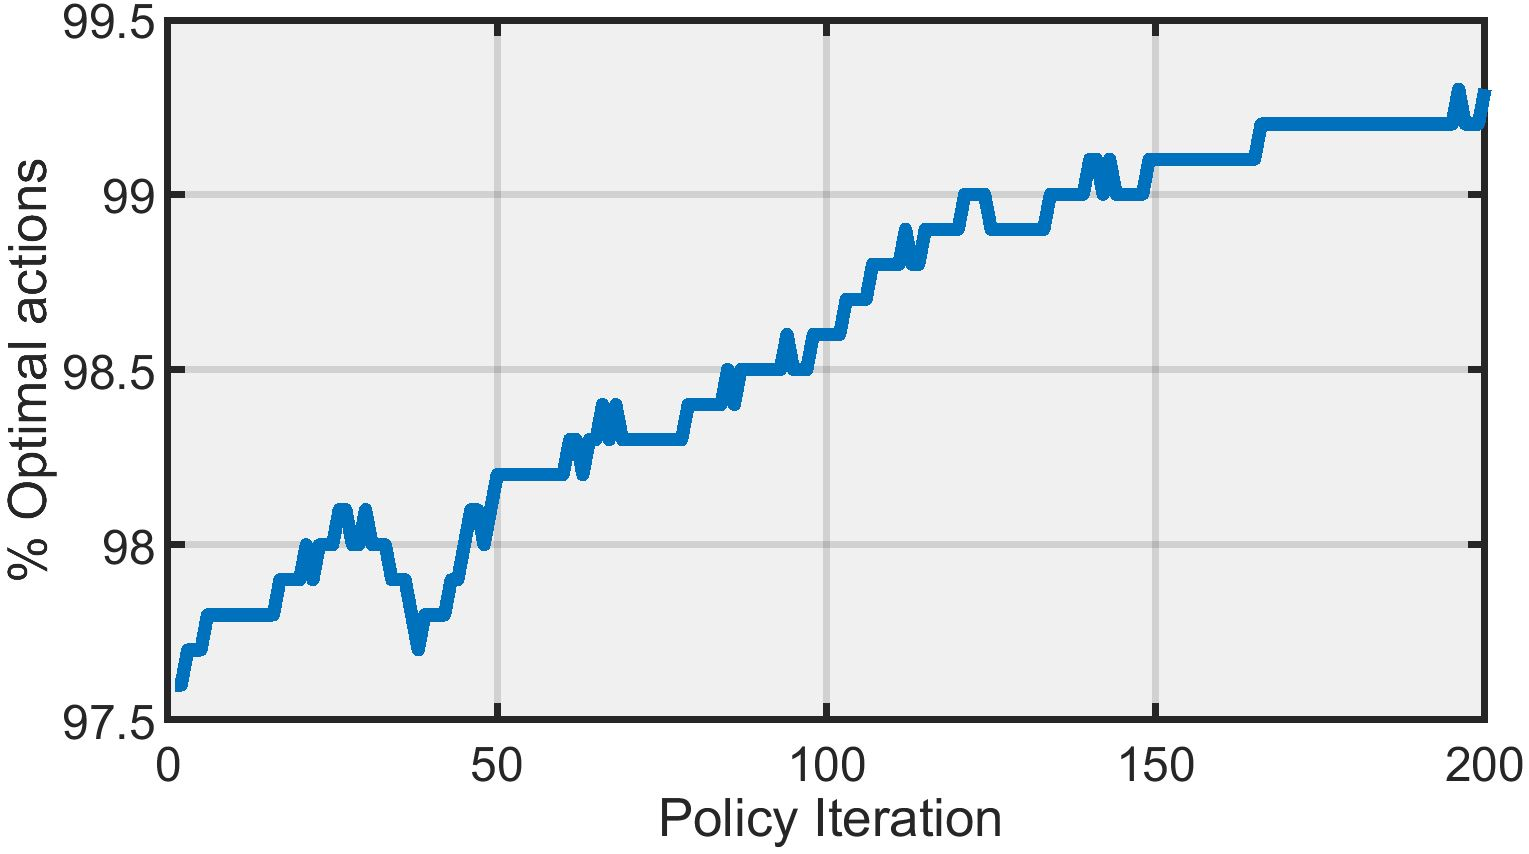
\includegraphics[ height=0.2\textwidth, width=0.35\textwidth]{Paper_IL_opt}
     }
     \caption{Learning of optimal actions. Results for the criss-cross network of Figure \ref{fig:cc} under different
traffic regimes.}
     \label{fig:cc_opt}
   \end{figure}


\begin{figure}[H]
    \subfloat[6-classes network \label{subfig-6:IL}]{%
       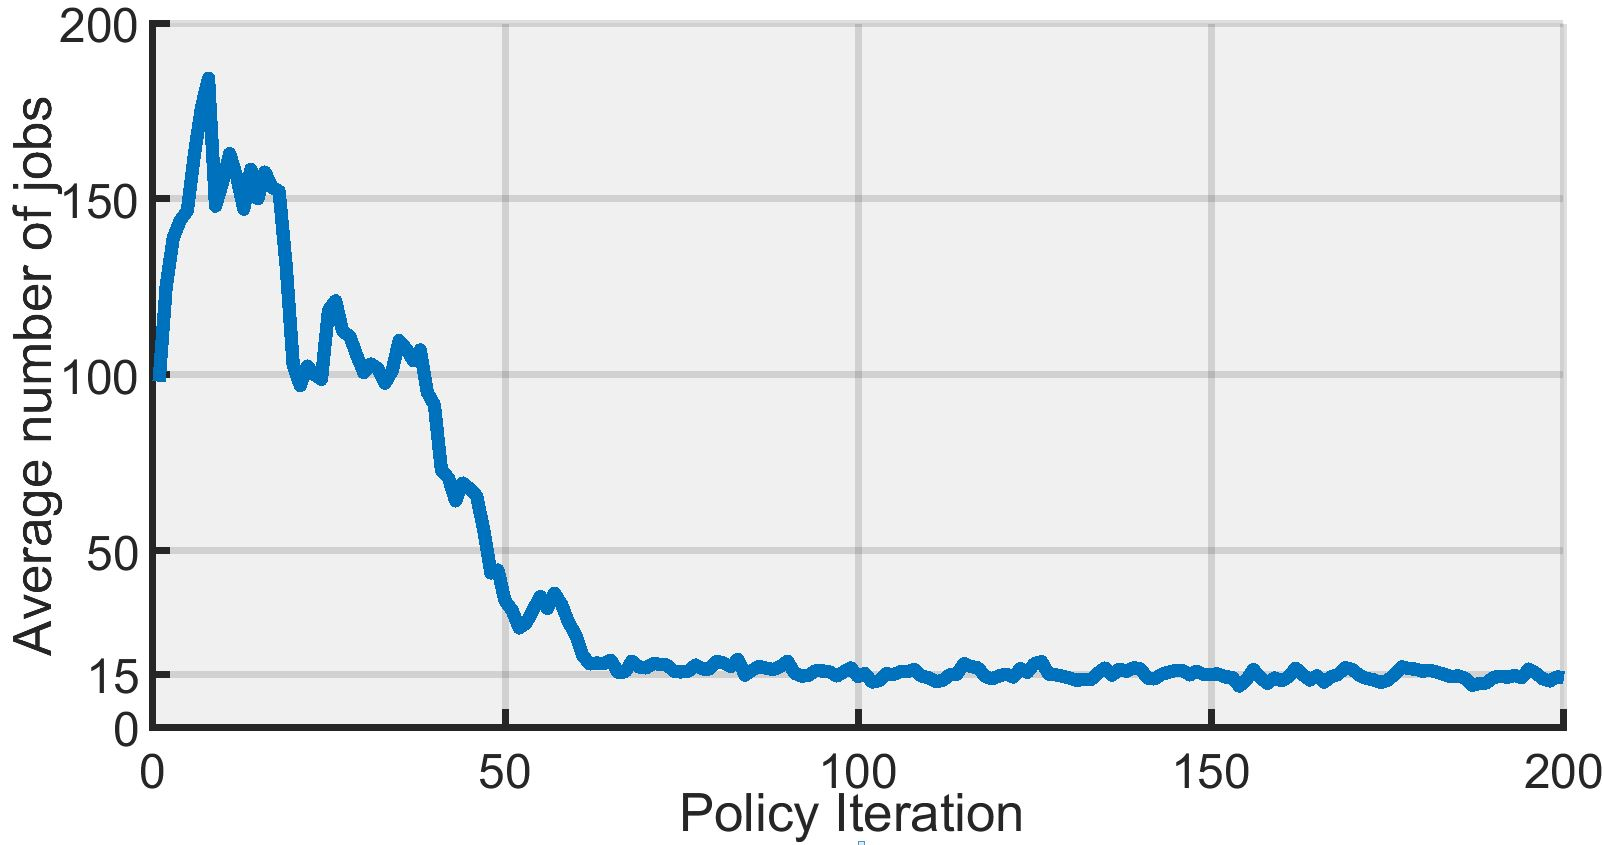
\includegraphics[height=0.2\textwidth, width=0.35\textwidth]{Paper6classes}
     }
     \subfloat[9-classes network \label{subfig-4:IM}]{%
       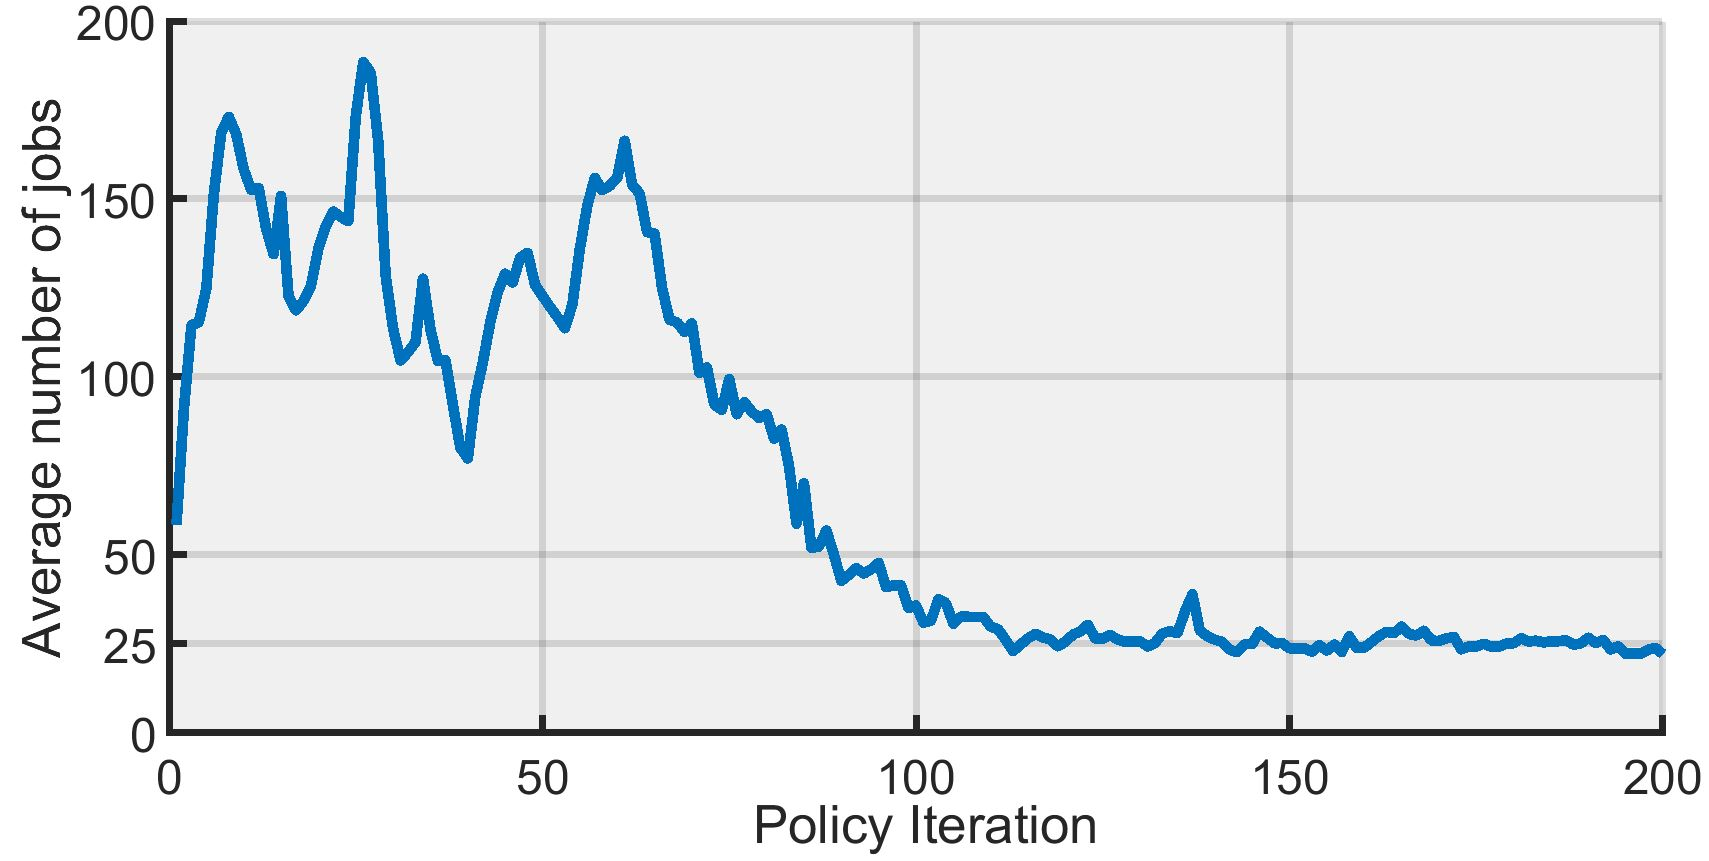
\includegraphics[height=0.2\textwidth, width=0.35\textwidth]{Paper9classes}
     }
     \subfloat[12-classes network \label{subfig-2:IH}]{%
       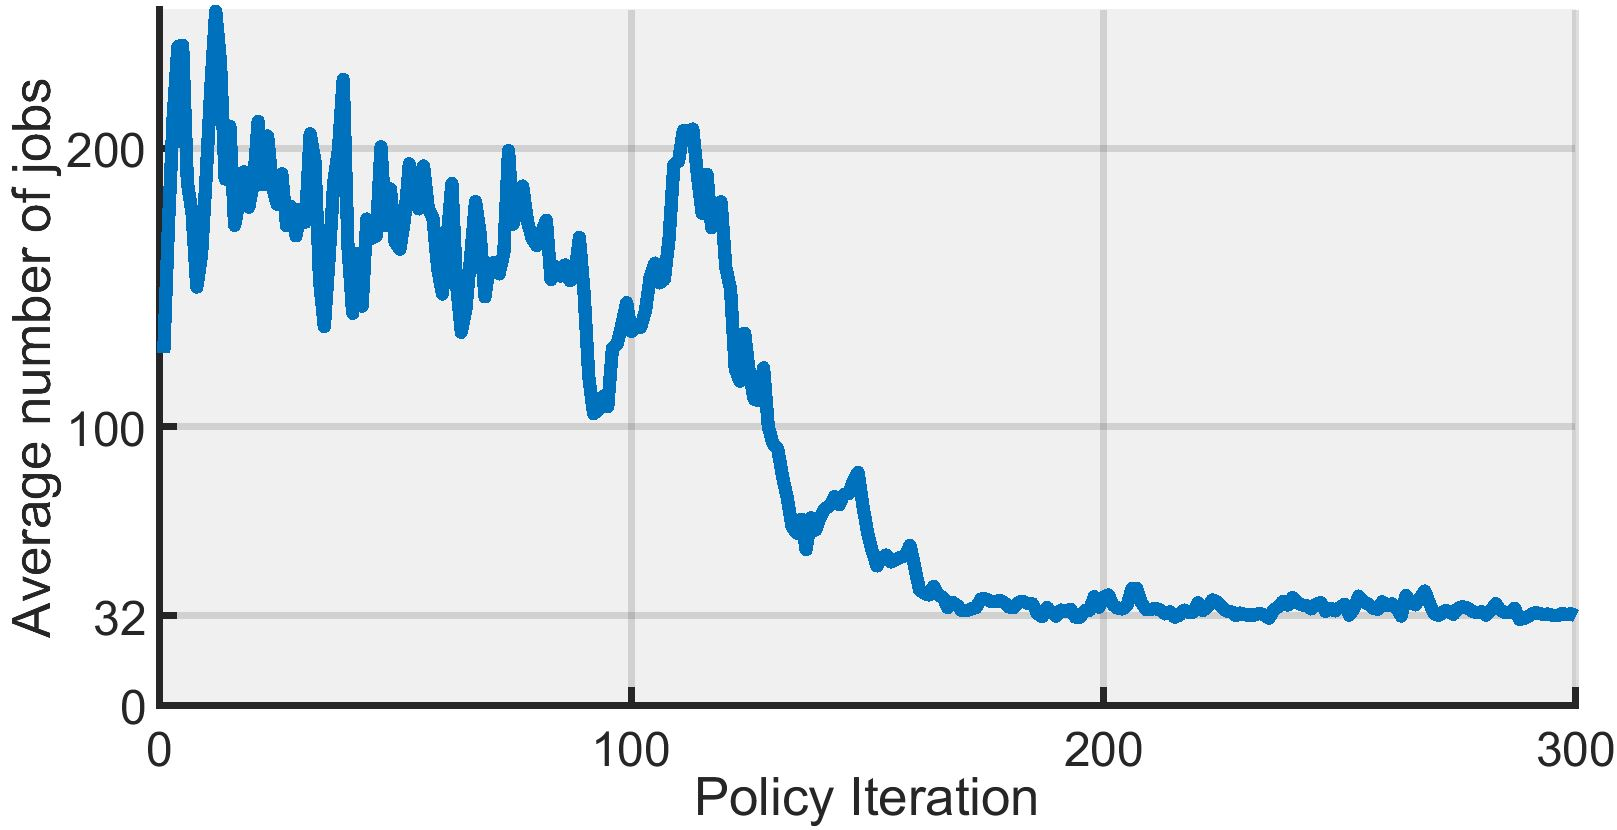
\includegraphics[height=0.2\textwidth, width=0.35\textwidth]{Paper12classes}
     }\\
 \subfloat[15-classes network\label{subfig-5:BL}]{%
       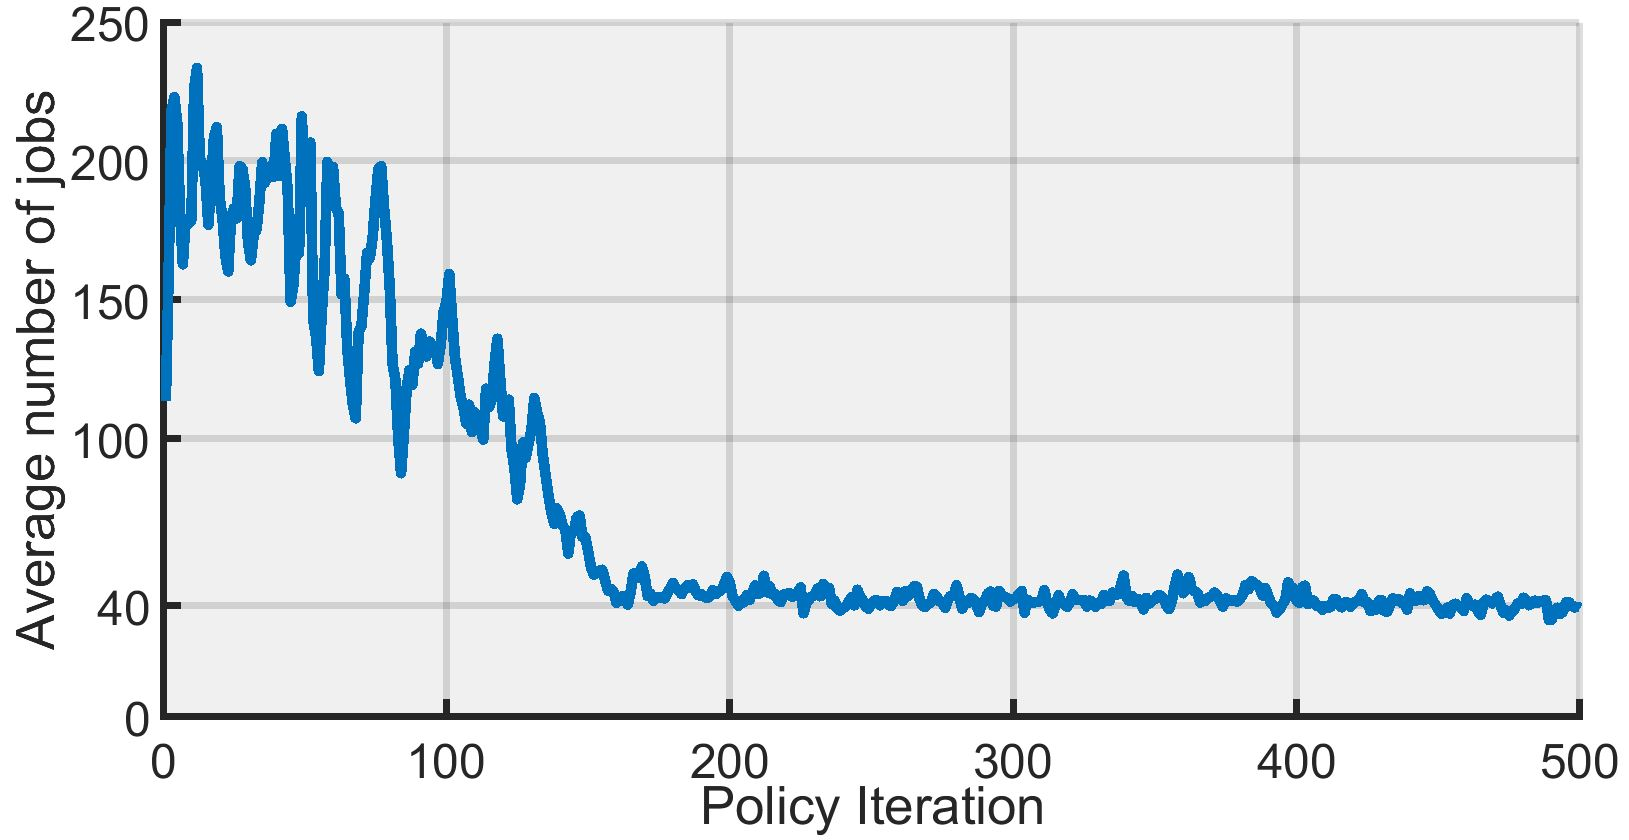
\includegraphics[ height=0.2\textwidth, width=0.35\textwidth]{Paper15classes}
     }
  \subfloat[18-classes network\label{subfig-3:BM}]{%
       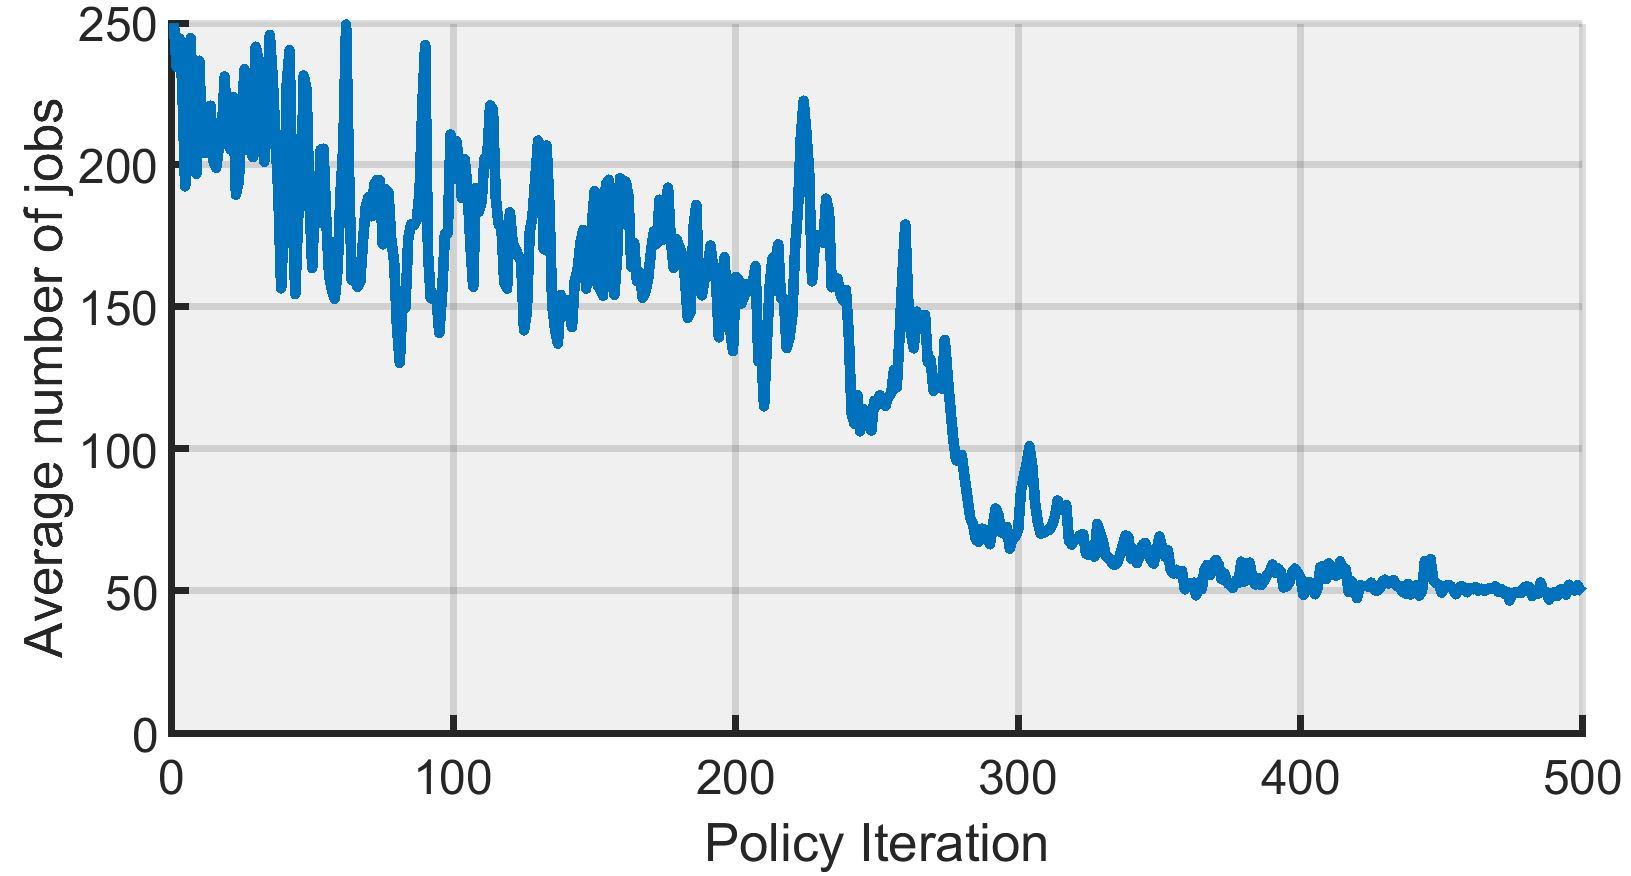
\includegraphics[ height=0.2\textwidth, width=0.35\textwidth]{Paper18classes}
     }
     \subfloat[21-classes network\label{subfig-1:BH}]{%
       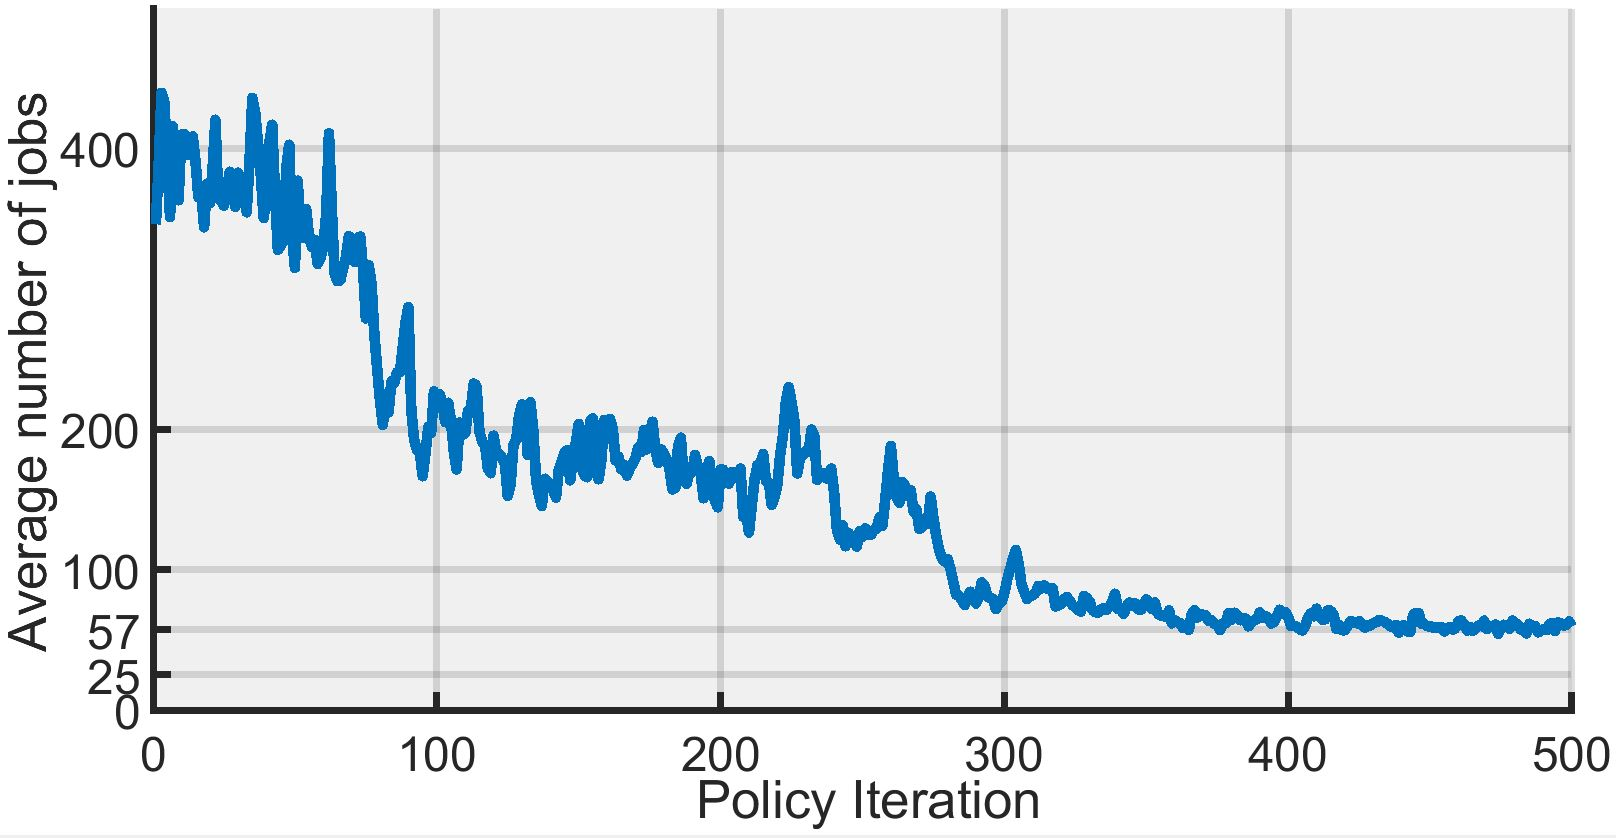
\includegraphics[ height=0.2\textwidth, width=0.35\textwidth]{Paper21classes}
     }


\caption{Learning curves for the 6-class extended network of Figure \ref{fig1}}
     \label{fig:ext_ac}
   \end{figure}


\begin{figure}[H]
    \subfloat[6-classes network \label{subfig-6:IL}]{%
       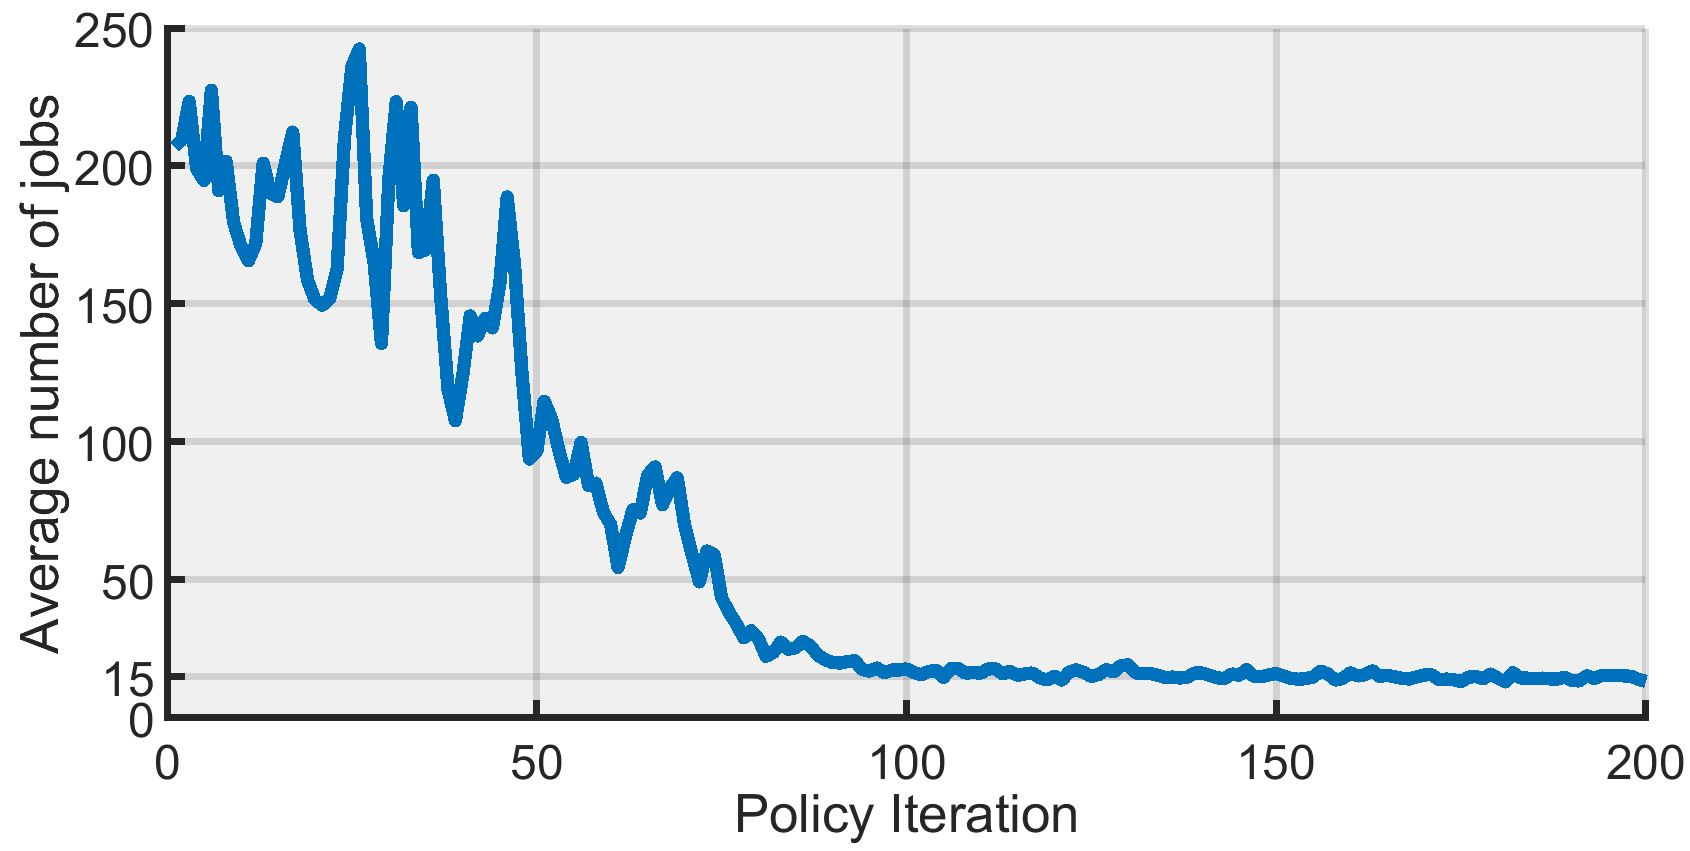
\includegraphics[height=0.2\textwidth, width=0.35\textwidth]{Paper6classes_re}
     }
     \subfloat[9-classes network \label{subfig-4:IM}]{%
       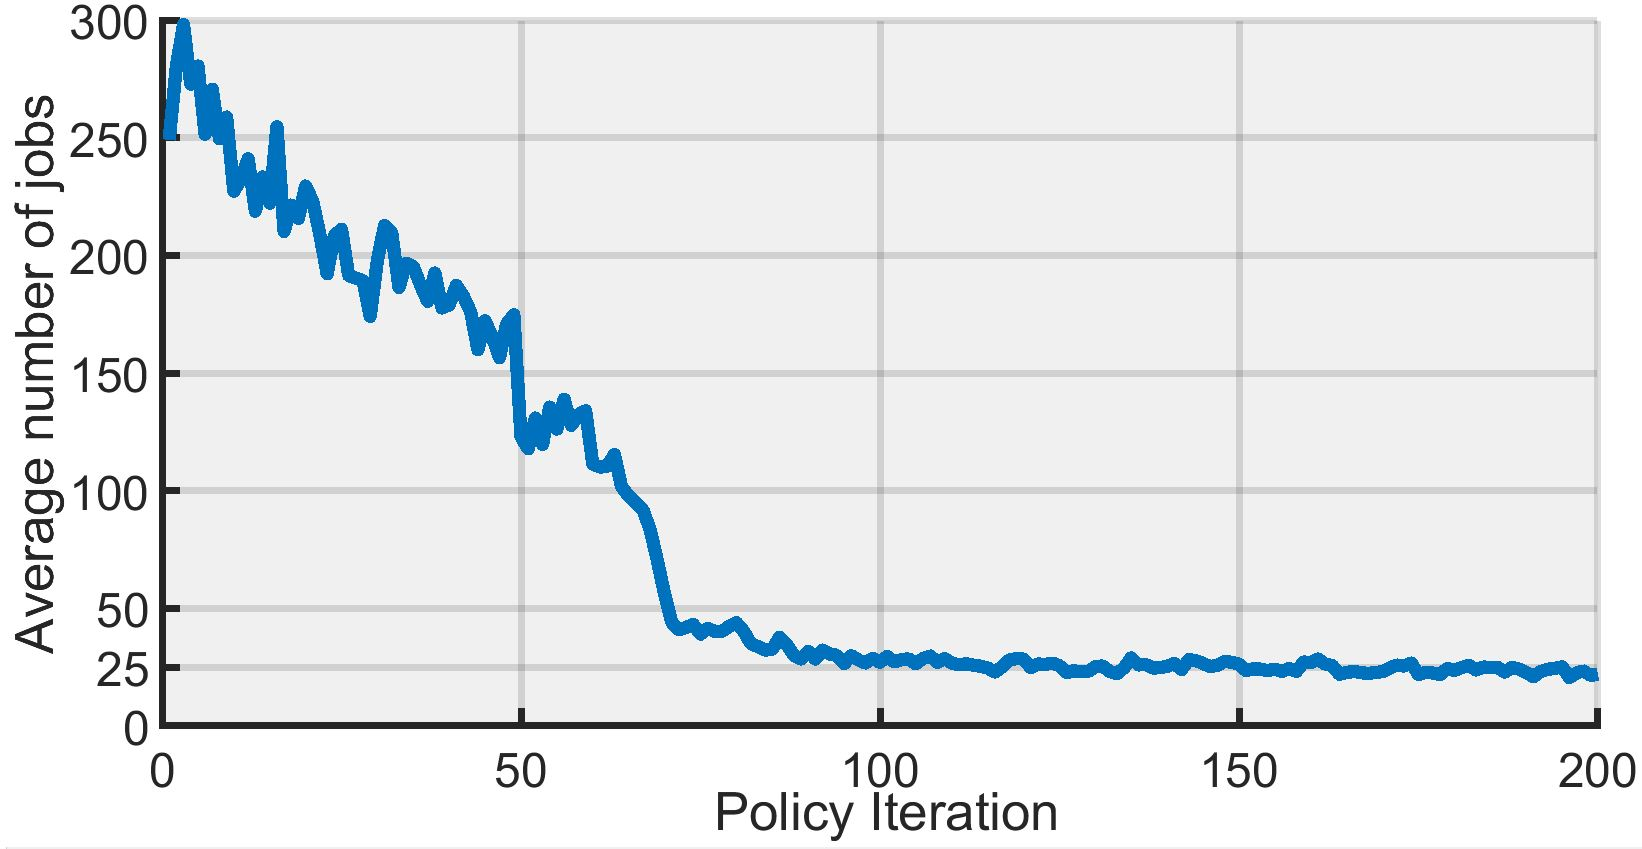
\includegraphics[height=0.2\textwidth, width=0.35\textwidth]{Paper9classes_re}
     }
     \subfloat[12-classes network \label{subfig-2:IH}]{%
       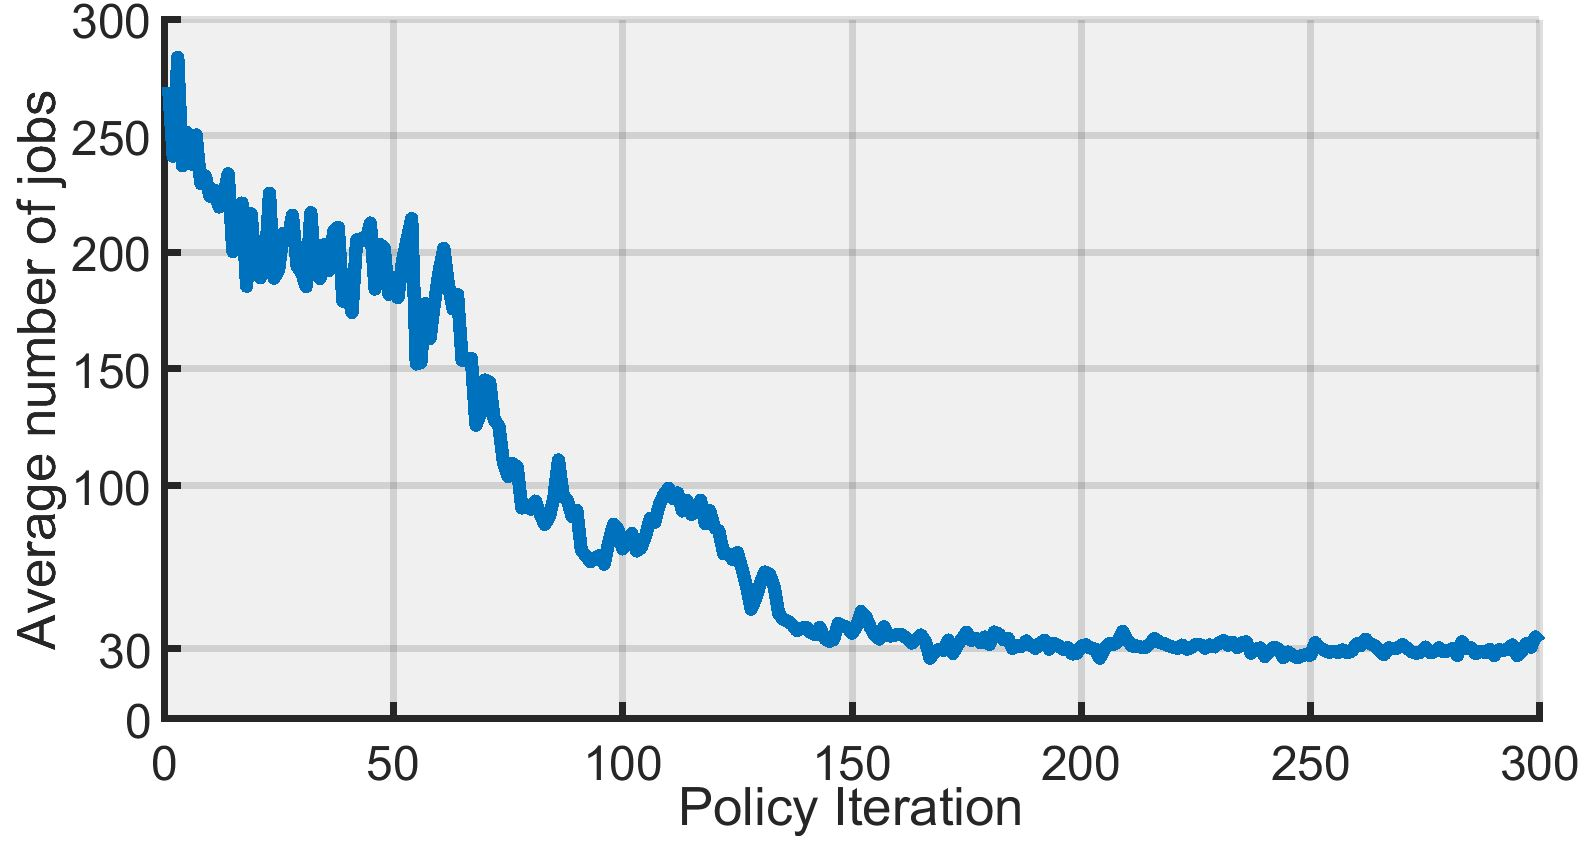
\includegraphics[height=0.2\textwidth, width=0.35\textwidth]{Paper12classes_re}
     }\\
 \subfloat[15-classes network\label{subfig-5:BL}]{%
       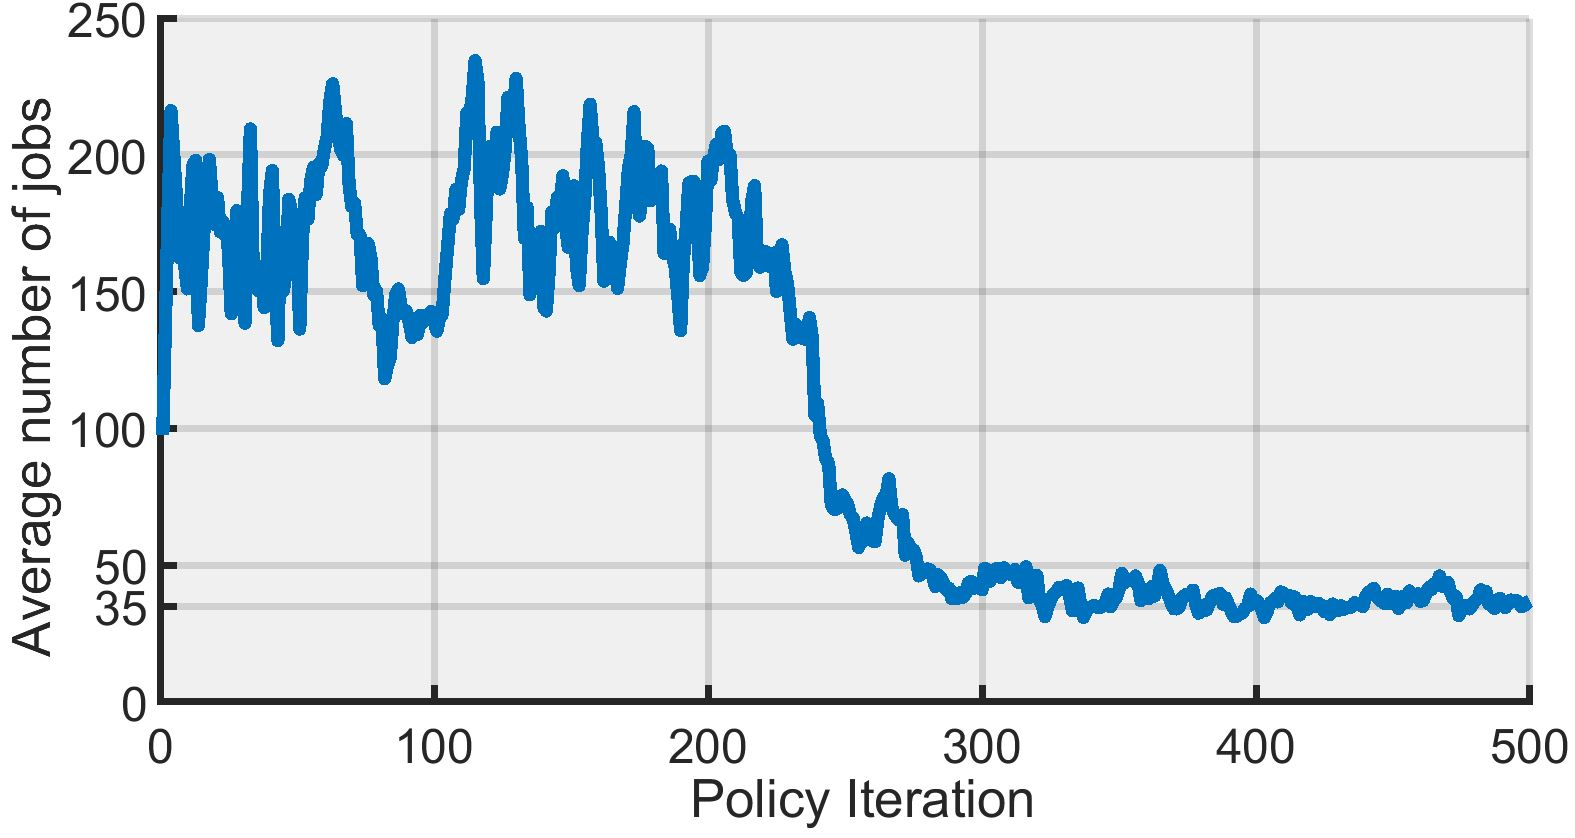
\includegraphics[ height=0.2\textwidth, width=0.35\textwidth]{Paper15classes_re}
     }
  \subfloat[18-classes network\label{subfig-3:BM}]{%
       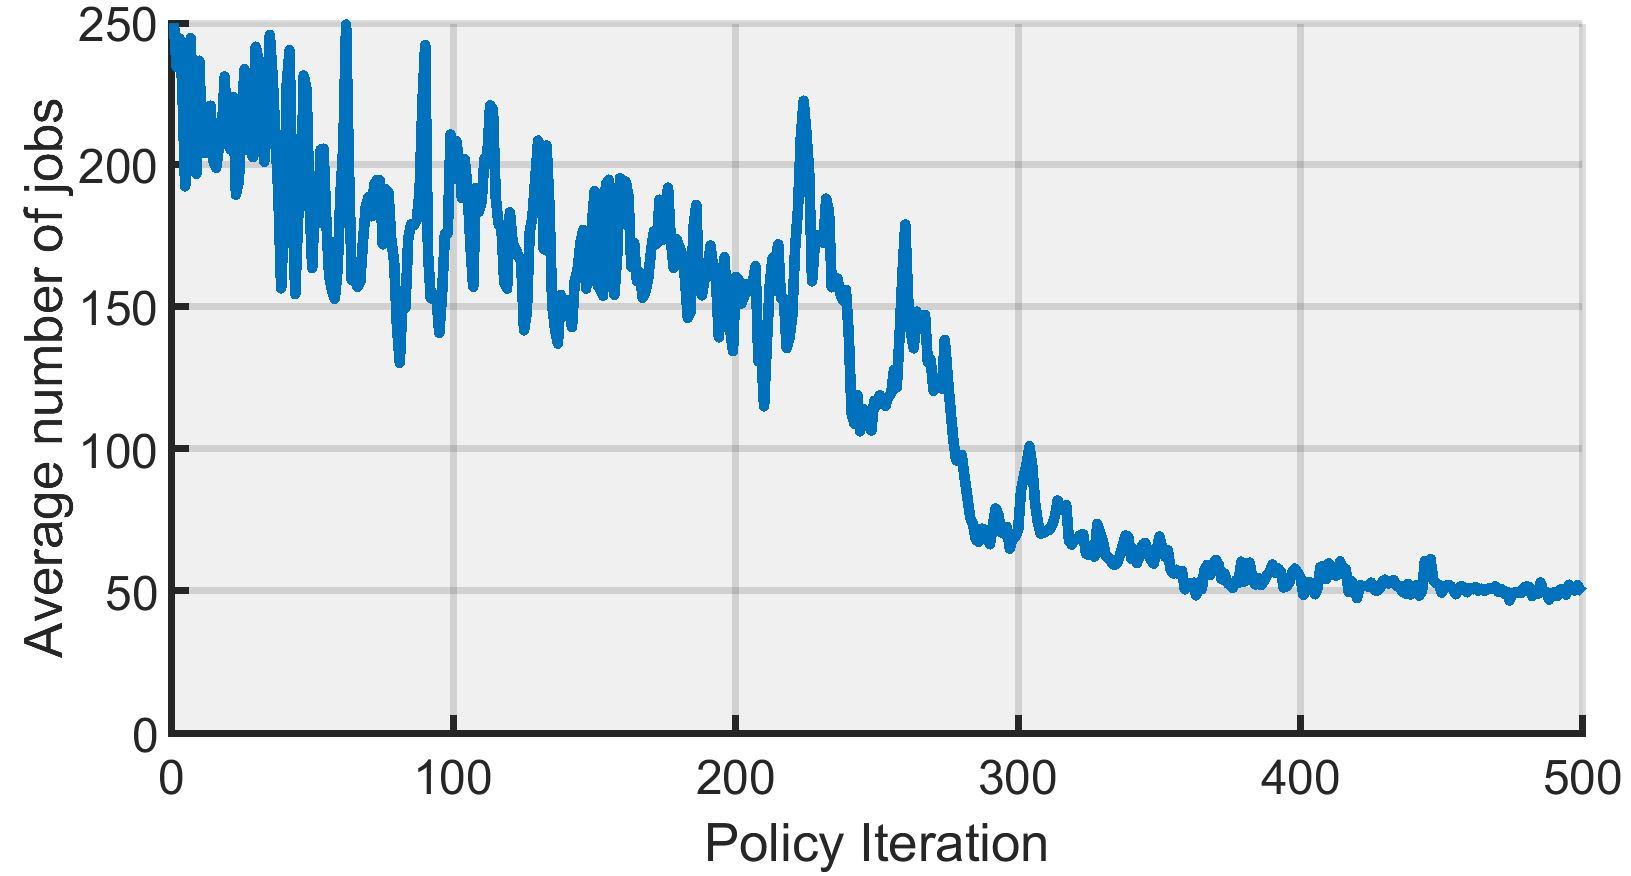
\includegraphics[ height=0.2\textwidth, width=0.35\textwidth]{Paper18classes}
     }
     \subfloat[21-classes network\label{subfig-1:BH}]{%
       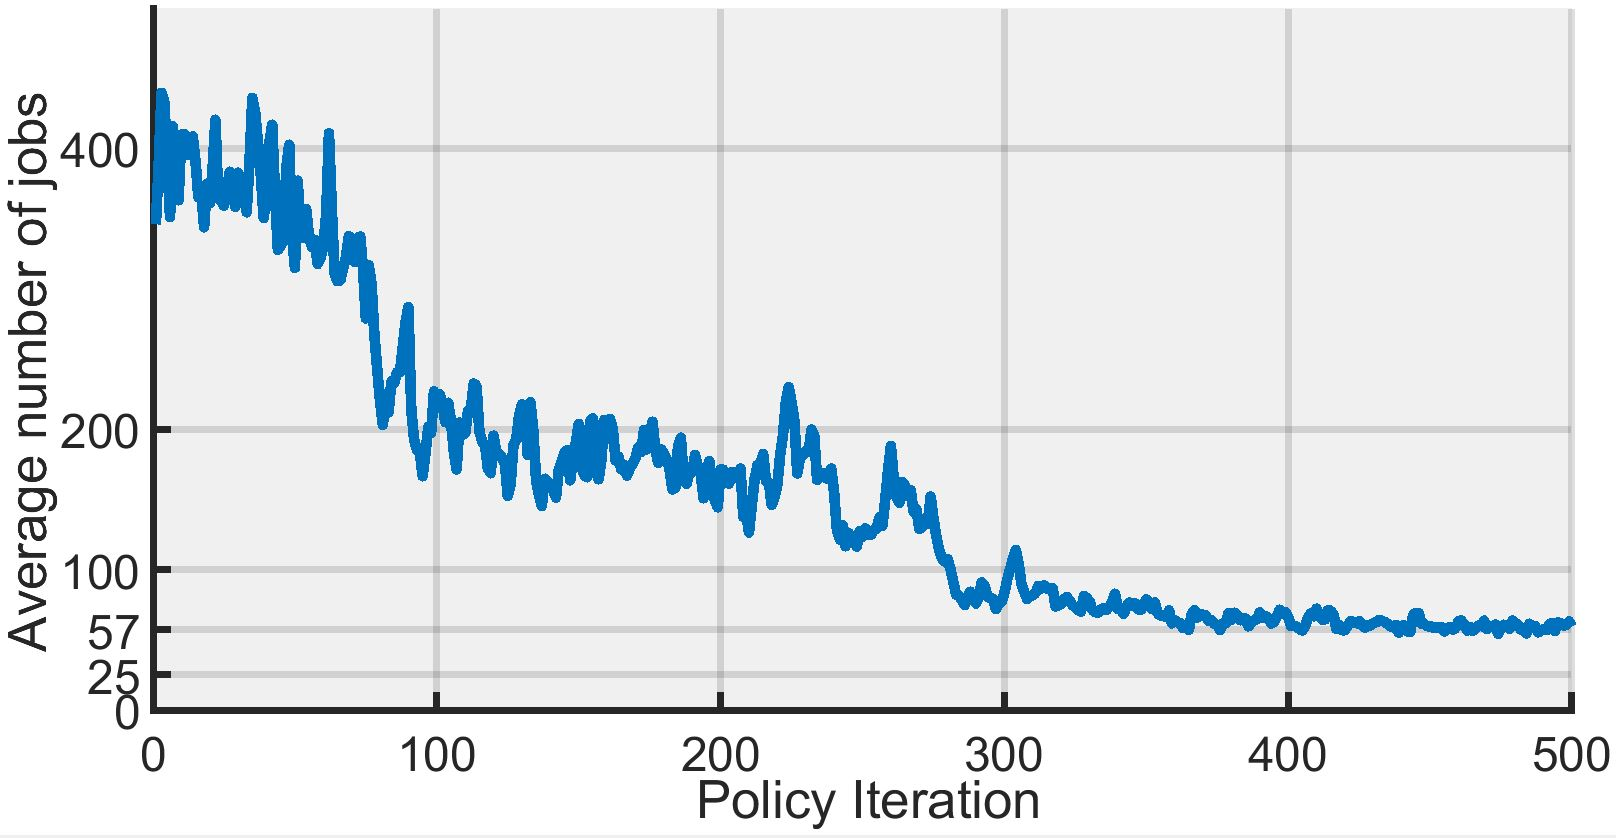
\includegraphics[ height=0.2\textwidth, width=0.35\textwidth]{Paper21classes}
     }


\caption{Learning curves for the reentrant extended network of Figure \ref{fig2}}
     \label{fig:reent_ac}
   \end{figure}
   
   
   \subsection{Implementation Details}
   
   We use Tensorflow v1.13.1 framework \cite{Abadi2016} to build a training routine of the neural networks and Ray package v0.6.3 \cite{Moritz2018} to maintain parallel simulation of actors. All experiments have been proceeded on a   2.1 GHz  32-core processor with 125 GB of RAM. We note that in most of our experiments we used $N=50$ actors that approximately double simulation time.
   
   
   \begin{table}[H]
\centering%
\begin{tabular}{|c|c|}
  \hline
  % after \\: \hline or \cline{col1-col2} \cline{col3-col4} ...
  Num. of classes $3L$  & Time, minutes  \\\hline
  6 & 0.75 \\\hline
  9 & 0.78 \\\hline
  12  & 1.07\\\hline
  15  & 1.54 \\\hline
  18  & 2.11\\\hline
  21  & 2.61 \\
  \hline
\end{tabular}
\caption[]{Running time of one policy iteration of the RL algorithm for the extended six-class network of Figure \ref{fig1}.}\label{tab:rt}
\end{table}



\bibliographystyle{plain}
\bibliography{PPO}



\end{document}   